\documentclass[12pt, a4paper]{mwrep}

\usepackage[utf8]{inputenc}							%kodowanie znaków
\usepackage[T1]{fontenc}								%kodowanie fontu
\usepackage{polski}									%polskie wcięcia itp
\usepackage{graphicx}								%wstawianie grafik
\usepackage{booktabs}								%scalanie kolumn
\usepackage{enumitem}								%lista a), b), c)
\usepackage{multirow}								%scalanie komórek tabeli w pionie
\usepackage{listings}								%wklejanie kodu z SQL
\usepackage{xcolor}									%żeby kolory do kodu działaly
\usepackage[margin=0.5in]{geometry}					%zmiana marginesów
\usepackage[hidelinks]{hyperref}						%linki w spisie treści

\hypersetup{linktoc=all}								%ustawienie linków w spisie treści
\linespread{1.3}										%interlinia 1,5

\lstdefinestyle{SQLStyle}{
                language=SQL,
                numbers=left,
                frame=single,
                basicstyle=\ttfamily,
                keywordstyle=\color{blue}\ttfamily,
                stringstyle=\color{red}\ttfamily,
                commentstyle=\color{green}\ttfamily,
                morecomment=[l][\color{magenta}]{\#},
                showstringspaces=false}

\lstdefinestyle{PythonStyle}{
                language=Python,
                numbers=left,
                frame=single,
                basicstyle=\ttfamily\small,
                keywordstyle=\color{blue}\ttfamily,
                stringstyle=\color{red}\ttfamily,
                commentstyle=\color{green}\ttfamily,
                morecomment=[l][\color{magenta}]{\#},
                showstringspaces=false}

\renewcommand{\maketitle}{

\newpage
\thispagestyle{empty} 

\begin{center}

\vspace*{1.5cm}


\includegraphics[scale=0.6]{pictures/agh.jpg}

\vspace*{0.5cm}

\large{\textsc{Wydział Informatyki, Elektroniki i~Telekomunikacji}}

\vspace*{0.5cm}

\normalsize{\textsc{Podstawy baz danych}}

\vspace*{0.75cm}

\LARGE{\textbf{System zarządzania konferencjami}}

\vspace*{0.25cm}

\large{\textbf{Dokumentacja projektu}}

\vspace*{1cm}

\normalsize{\textit{Autor:}}

\normalsize{\textsc{Piotr Wróbel}}

\vspace*{1cm}

\textit{Opieka nad projektem:}

\textsc{dr~inż.~Robert Marcjan}

\vfill

\small{\textit{semestr zimowy 2018/19}}

\end{center}

\newpage
}

\begin{document}

\maketitle

\tableofcontents

\chapter{Opis funkcji systemu}

Przedstawiony projekt ma na celu stworzenie bazy danych wspomagającej działalność firmy organizującej konferencje. Rejestracja organizowana jest poprzez stronę internetową, klientami mogą być zarówno osoby prywatne jak i~firmy. Możliwa jest zbiorcza rezerwacja wielu miejsc z~podaniem danych uczestników w~późniejszym terminie. Dla konferencji wielodniowych nie ma konieczności zapisywania się na cały ich przebieg i~dla każdej osoby biorącej w~nich udział istnieje możliwość indywidualnego wyboru poszczególnych dni oraz warsztatów (jeżeli takie są organizowane).

\section{Funkcjonalności systemu}

Do aktorów korzystających z~systemów należą administrator systemu, organizator konferencji oraz klient (indywidualny bądź firma) o~następujących funkcjonalnościach:

\subsection{Administrator systemu}

\begin{itemize}
  \item Przydzielanie uprawnień pozostałym użytkownikom
  \item Pełen dostęp do bazy danych
\end{itemize}

\subsection{Organizator konferencji}

\begin{itemize}
  \item Dodanie nowej konferencji wraz z~jej nazwą, terminem, liczbą dni, terminami ewentualnych warsztatów, obowiązującymi progami cenowymi i~zniżkami studenckimi, limitem miejsc na poszczególne dni/warsztaty oraz miejscem odbywania się konferencji
  \item Wyświetlenie listy wszystkich klientów
  \item Wyświetlenie listy wszystkich uczestników danej konferencji z~możliwością sporządzenia jej tylko dla poszczególnych dni lub warsztatów
  \item Dostęp do danych o~płatnościach, możliwość anulowania nieopłaconej rezerwacji
  \item Możliwość modyfikacji danych konferencji wraz z~wymuszeniem konsekwencji zmian (np.~w~przypadku zmiany liczby miejsc na konkretny warsztat)
  \item Uniemożliwienie klientowi rejestracji na kolidujące ze sobą warsztaty
  \item Generowanie raportu statystycznego na temat klientów, którzy najczęściej korzystają z~usług danego organizatora
\end{itemize}

\subsection{Klient}

\begin{itemize}
  \item Prezentowanie informacji o~konferencji: jej nazwy, dni, odbywających się warsztatów oraz poszczególnych cen
  \item Rezerwacja określonej ilości miejsc na wybrane dni, bez konieczności podawania danych uczestników 
  \item Rejestracja uczestników na warsztaty
  \item Modyfikacja danych rezerwacji w~zakresie ilości miejsc, przydziału dni lub warsztatów
  \item Uzupełnienie danych osobowych uczestników w~odpowiednim terminie
  \item Udostępnienie informacji o~historii płatności związanych z~daną konferencją i~pozostałą do zapłaty kwotą
\end{itemize}

\lstset{style=SQLStyle}

\chapter{Schemat bazy danych}

\section{Diagram bazy danych}

\begin{figure}[h]
  \centering
  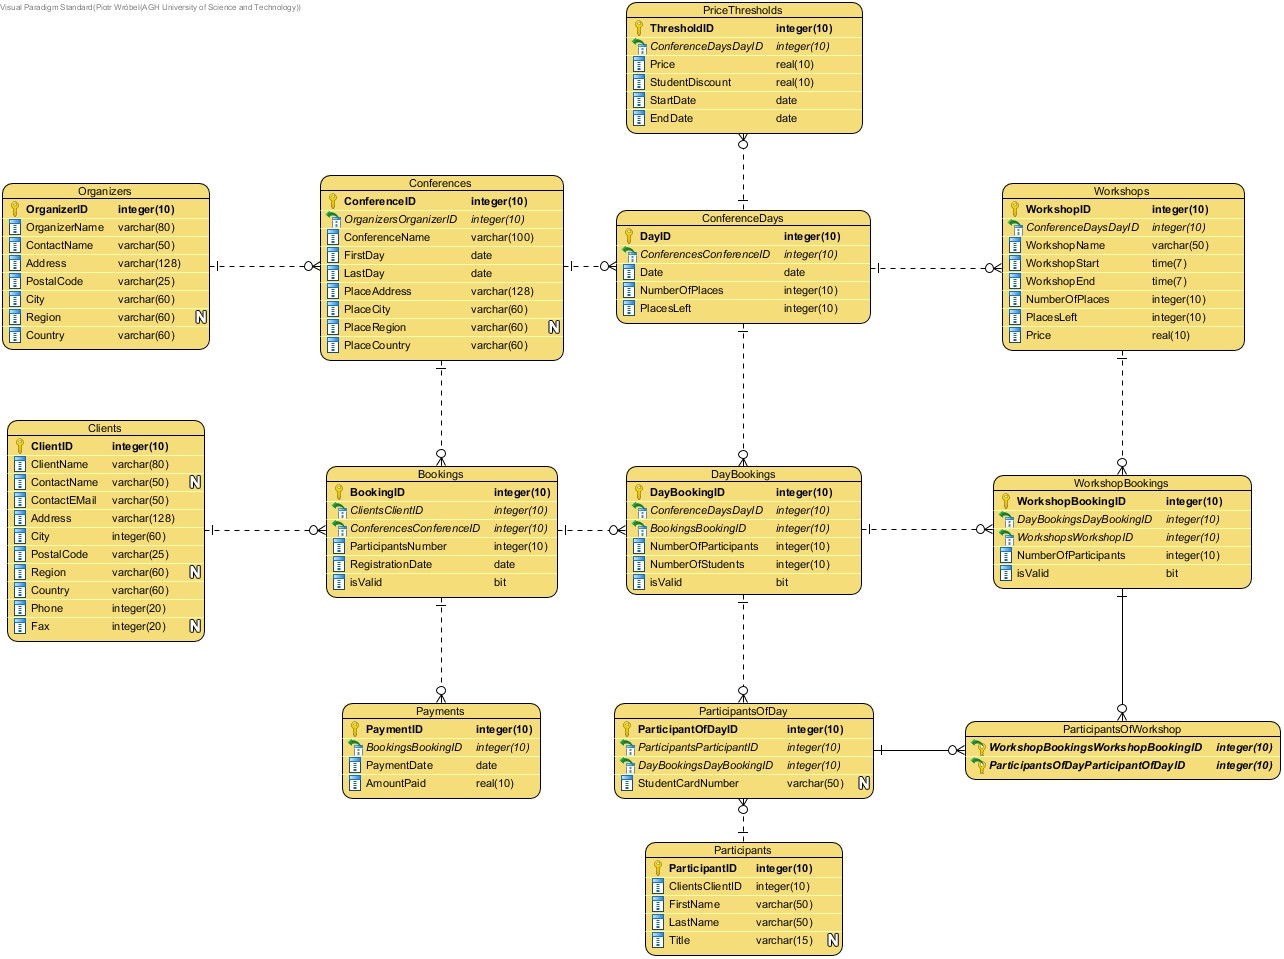
\includegraphics[width=0.99\textwidth]{pictures/scheme.jpg}
  \caption{Schemat projektowanej bazy danych wykonany w~programie Visual Paradigm}
  \label{rys:schemat}
\end{figure}

\newpage
\section{Opis tabel}

\subsection{Tabela Organizers}

\noindent Zawiera dane organizatorów konferencji \ppauza nazwę organizatora, dane osoby kontaktowej i~adres.

\vspace{0.5cm}

\noindent \textbf{Pola tabeli:}
\begin{itemize}
  \item \textbf{OrganizerID} \ppauza identyfikator organizatora, \textbf{klucz główny}
  \item \textbf{OrganizerName} \ppauza nazwa organizatora
  \item \textbf{ContactName} \ppauza imię i~nazwisko osoby kontaktowej
  \item \textbf{Address} \ppauza ulica i~numer lokalu organizatora
  \item \textbf{Postal Code} \ppauza kod pocztowy
  \item \textbf{City} \ppauza miasto
  \item \textbf{Region} \ppauza województwo/stan (jeśli dotyczy, inaczej pole ma wartoć null)
  \item \textbf{Country} \ppauza kraj
\end{itemize}

\vspace{0.5cm}
\noindent \textbf{Kod SQL generujący tabelę:}

\begin{lstlisting}
create table Organizers (
  OrganizerID           int not null identity,
  OrganizerName         nvarchar(80) not null,
  ContactName           nvarchar(50) not null,
  Address               nvarchar(128) not null,
  PostalCode            nvarchar(25) not null,
  City                  nvarchar(60) not null,
  Region                nvarchar(60) default null,
  Country               nvarchar(60) not null,
  constraint PK_Organizers 
    primary key (OrganizerID)
)
\end{lstlisting}

\vspace{0.5cm}
\noindent \textbf{Warunki integralnościowe}
\begin{itemize}
  \item pole OrganizerID jest kluczem głównym
  \item wszystkie pola poza Region nie mogą mieć wartości pustej
\end{itemize}

\newpage
\subsection{Tabela Conferences}

\noindent Zawiera dane konferencji \ppauza jej nazwę, dni w~których się odbywa oraz dane adresowe miejsca

\vspace{0.5cm}

\noindent \textbf{Pola tabeli:}
\begin{itemize}
  \item \textbf{ConferenceID} \ppauza identyfikator konferencji, \textbf{klucz główny}
  \item \textbf{OrganizerID} \ppauza identyfikator organizatora konferencji, \textbf{klucz obcy}
  \item \textbf{ConferenceName} \ppauza nazwa konferencji
  \item \textbf{FirstDay} \ppauza pierwszy dzień konferencji
  \item \textbf{LastDay} \ppauza ostatni dzień konferencji
  \item \textbf{PlaceAddress} \ppauza ulica i~numer lokalu miejsca, w~którym odbywa się konferencja
  \item \textbf{PlaceCity} \ppauza miasto, w~którym odbywa się konferencja
  \item \textbf{PlaceRegion} \ppauza województwo/stan, w~którym odbywa się konferencja
  \item \textbf{PlaceCountry} \ppauza kraj, w~którym odbywa się konferencja
\end{itemize}

\vspace{0.5cm}
\noindent \textbf{Kod SQL generujący tabelę:}

\begin{lstlisting}
create table Conferences (
  ConferenceID          int not null identity,
  OrganizerID           int not null,
  ConferenceName        nvarchar(100) not null,
  FirstDay              date not null,
  LastDay               date not null,
  PlaceAddress          nvarchar(128) not null,
  PlaceCity             nvarchar(60) not null,
  PlaceRegion           nvarchar(60) default null,
  PlaceCountry          nvarchar(60) not null,
  constraint PK_Conferences 
    primary key (ConferenceID),
  constraint Conferences_Organizers 
    foreign key (OrganizerID) 
    references Organizers (OrganizerID),
  constraint CK_LastDay_FirstDay_Conferences 
    check (LastDay >= FirstDay)
)
\end{lstlisting}

\vspace{0.5cm}

\noindent \textbf{Warunki integralnościowe}
\begin{itemize}
  \item pole ConferenceID jest kluczem głównym
  \item pole OrganizerID jest kluczem obcym
  \item wszystkie pola poza PlaceRegion muszą być niepuste
  \item data zapisana w~polu LastDay nie może być wcześniejsza niż ta z~FirstDay
\end{itemize}

\newpage
\subsection{Tabela Clients}

\noindent Zawiera dane klientów firmowych jak i~indywidualnych

\vspace{0.5cm}

\noindent \textbf{Pola tabeli:}
\begin{itemize}
  \item \textbf{ClientID} \ppauza identyfikator klienta, \textbf{klucz główny}
  \item \textbf{ClientName} \ppauza nazwa klienta firmowego/imię i~nazwisko klienta indywidualnego
  \item \textbf{ContactName} \ppauza imię i~nazwisko osoby kontaktowej dla klientów firmowych
  \item \textbf{ContactEMail} \ppauza adres e\dywiz{}mailowy klienta
  \item \textbf{Address} \ppauza ulica i~numer lokalu klienta
  \item \textbf{City} \ppauza miasto zamieszkania klienta
  \item \textbf{PostalCode} \ppauza kod pocztowy klienta
  \item \textbf{Region} \ppauza stan/województwo zamieszkania klienta
  \item \textbf{Country} \ppauza kraj zamieszkania klienta
  \item \textbf{Phone} \ppauza telefon do klienta
  \item \textbf{Fax} \ppauza fax klienta
\end{itemize}

\vspace{0.5cm}
\noindent \textbf{Kod SQL generujący tabelę:}

\begin{lstlisting}
create table Clients (
  ClientID              int not null identity,
  ClientName            nvarchar(80) not null,
  ContactName           nvarchar(50) default null,
  ContactEMail          nvarchar(50) not null check
    (ContactEMail like '%_@_%._%'),
  Address               nvarchar(128) not null,
  City                  nvarchar(60) not null,
  PostalCode            nvarchar(25) not null,
  Region                nvarchar(60) default null,
  Country               nvarchar(60) not null,
  Phone                 varchar(20) not null,
  Fax                   varchar(20) default null,
  constraint PK_Clients 
    primary key (ClientID)
)
\end{lstlisting}

\vspace{0.5cm}
\noindent \textbf{Warunki integralnościowe}
\begin{itemize}
  \item pole ClientID jest kluczem głównym
  \item pola ClientName, ClientEMail, Address, City, PostalCode, Country, Phone nie mogą być puste, pozostałe są uzupełniane w~razie potrzeby (np.~dla klienta firmowego pole ContactName)
  \item pole ContactEMail musi mieć określony format
\end{itemize}

\subsection{Tabela Bookings}

\noindent Zawiera dane rezerwacji wykonanych przez klientów

\vspace{0.5cm}

\noindent \textbf{Pola tabeli:}
\begin{itemize}
  \item \textbf{BookingID} \ppauza identyfikator rezerwacji, \textbf{klucz główny}
  \item \textbf{ClientID} \ppauza identyfikator klienta, który wykonał rezerwację, \textbf{klucz obcy}
  \item \textbf{ConferenceID} \ppauza identyfikator konferencji, na którą wykonano rezerwację, \textbf{klucz obcy}
  \item \textbf{ParticipantsNumber} \ppauza liczba osób, dla których wykonywana jest rezerwacja
  \item \textbf{RegistrationDate} \ppauza data wykonania rezerwacji
  \item \textbf{isValid} \ppauza czy rezerwacja jest ważna
\end{itemize}

\vspace{0.5cm}
\noindent \textbf{Kod SQL generujący tabelę:}

\begin{lstlisting}
create table Bookings (
  BookingID             int not null identity,
  ClientID              int not null,
  ConferenceID          int not null,
  ParticipantsNumber    int not null check
    (ParticipantsNumber > 0),
  RegistrationDate      datetime not null default getdate(),
  isValid               bit not null default 1,
  constraint PK_Bookings 
    primary key (BookingID),
  constraint Bookings_Clients 
    foreign key (ClientID) 
    references Clients (ClientID),
  constraint Bookings_Conferences 
    foreign key (ConferenceID) 
    references Conferences (ConferenceID)
)

\end{lstlisting}

\vspace{0.5cm}
\noindent \textbf{Warunki integralnościowe}
\begin{itemize}
  \item pole BookingID jest kluczem głównym
  \item pola ClientID i~ConferenceID są kluczami obcymi
  \item pozostałe pola muszą być niepuste
  \item pole ParticipantsNumber musi zawierać liczbę większą od~0
\end{itemize}

\newpage
\subsection{Tabela Payments}

\noindent Zawiera dane dotyczące płatności wykonanych dla danej rezerwacji

\vspace{0.5cm}

\noindent \textbf{Pola tabeli:}
\begin{itemize}
  \item \textbf{PaymentID} \ppauza identyfikator płatności, \textbf{klucz główny}
  \item \textbf{BookingID} \ppauza identyfikator rezerwacji, \textbf{klucz obcy}
  \item \textbf{PaymentDate} \ppauza data wykonania płatności
  \item \textbf{AmountPaid} \ppauza zapłacona kwota
\end{itemize}

\vspace{0.5cm}
\noindent \textbf{Kod SQL generujący tabelę:}

\begin{lstlisting}
create table Payments (
  PaymentID             int not null identity ,
  BookingID             int not null,
  PaymentDate           datetime not null default getdate(),
  AmountPaid            money not null check
    (AmountPaid > 0),
  constraint PK_Payments 
    primary key (PaymentID),
  constraint Payments_Bookings 
    foreign key (BookingID) 
    references Bookings (BookingID)
)
\end{lstlisting}

\vspace{0.5cm}
\noindent \textbf{Warunki integralnościowe}
\begin{itemize}
  \item pole PaymentID jest kluczem głównym
  \item pole Booking ID jest kluczem obcym
  \item pozostałe pola muszą być niepuste
  \item pole AmountPaid musi zawierać liczbę większą od~0
\end{itemize}

\subsection{Tabela ConferenceDays}

\noindent Zawiera informacje dotyczące ilości miejsc na poszczególne dni konferencji

\vspace{0.5cm}

\noindent \textbf{Pola tabeli:}
\begin{itemize}
  \item \textbf{DayID} \ppauza identyfikator dnia, \textbf{klucz główny}
  \item \textbf{ConferenceID} \ppauza identyfikator konferencji, \textbf{klucz obcy}
  \item \textbf{Date} \ppauza data
  \item \textbf{NumberOfPlaces} \ppauza liczba miejsc na dany dzień
  \item \textbf{PlacesLeft} \ppauza pozostała liczba miejsc
\end{itemize}

\vspace{0.5cm}
\noindent \textbf{Kod SQL generujący tabelę:}

\begin{lstlisting}
create table ConferenceDays (
  DayID                 int not null identity,
  ConferenceID          int not null,
  Date                  date not null,
  NumberOfPlaces        int not null check
    (NumberOfPlaces > 0),
  PlacesLeft            int not null check
    (PlacesLeft >= 0),
  constraint PK_ConferenceDays 
    primary key (DayID),
  constraint ConferenceDays_Conferences 
    foreign key (ConferenceID) 
    references Conferences (ConferenceID),
  constraint CK_Places_ConferenceDays 
    check (PlacesLeft <= NumberOfPlaces),
  constraint Unique_Days_Conf 
    unique (ConferenceID, Date)
)
\end{lstlisting}

\vspace{0.5cm}
\noindent \textbf{Warunki integralnościowe}
\begin{itemize}
  \item pole DayID jest kluczem głównym
  \item pole ConferenceID jest kluczem obcym
  \item pole Date musi być niepuste, pozostałe organizator może uzupełnić w~późniejszym terminie
  \item pole NumberOfPlaces musi zawierać liczbę większą od~0
  \item pole PlacesLeft musi zawierać liczbę nie mniejszą od~0 i~nie większą od NumberOfPlaces, automatyczne ustawienie tej wartości zostanie rozwiązane za pomocą triggera
  \item każda para (ConferenceID, Date) musi być jedyna
\end{itemize}

\subsection{Tabela PriceThresholds}

\noindent Zawiera informacje dotyczące progów cenowych na poszczególne dni konferencji

\vspace{0.5cm}

\noindent \textbf{Pola tabeli:}
\begin{itemize}
  \item \textbf{ThresholdID} \ppauza identyfikator progu, \textbf{klucz główny}
  \item \textbf{DayID} \ppauza identyfikator dnia konferencji, \textbf{klucz obcy}
  \item \textbf{Price} \ppauza cena
  \item \textbf{StudentDiscount} \ppauza zniżka studencka (o~ile jest określana)
  \item \textbf{StartDate} \ppauza początek obowiązywania danego progu
  \item \textbf{EndDate} \ppauza koniec obowiązywania danego progu
\end{itemize}

\vspace{0.5cm}
\noindent \textbf{Kod SQL generujący tabelę:}

\begin{lstlisting}
create table PriceThresholds (
  ThresholdID           int not null identity,
  DayID                 int not null,
  Price                 money not null check
    (Price >= 0.0),
  StudentDiscount       real not null default 0 check
    (StudentDiscount between 0.0 and 100.0),
  StartDate             date not null,
  EndDate               date not null,
  constraint PK_PriceThresholds 
    primary key (ThresholdID),
  constraint PriceThresholds_ConferenceDays 
    foreign key (DayID) 
    references ConferenceDays (DayID),
  constraint CK_Dates_PriceThresholds 
    check (EndDate >= StartDate)
)
\end{lstlisting}

\vspace{0.5cm}
\noindent \textbf{Warunki integralnościowe}
\begin{itemize}
  \item pole ThresholdID jest kluczem głównym
  \item pole DayID jest kluczem obcym
  \item wszystkie pola muszą być niepuste
  \item zawartość pola Price musi być większa od~0
  \item zawartość pola StudentDiscount musi być między 0~a~100
  \item data zapisana w~EndDate musi być niewcześniejsza niż ta w~StartDate
\end{itemize}

\subsection{Tabela Workshops}

\noindent Zawiera informacje dotyczące warsztatów odbywających się w~poszczególnych dniach konferencji

\vspace{0.5cm}

\noindent \textbf{Pola tabeli:}
\begin{itemize}
  \item \textbf{WorkshopID} \ppauza identyfikator warsztatu, \textbf{klucz główny}
  \item \textbf{DayID} \ppauza identyfikator dnia konferencji, \textbf{klucz obcy}
  \item \textbf{WorkshopName} \ppauza nazwa warsztatu
  \item \textbf{WorkshopStart} \ppauza godzina rozpoczęcia
  \item \textbf{WorkshopEnd} \ppauza godzina zakończenia
  \item \textbf{NumberOfPlaces} \ppauza liczba miejsc
  \item \textbf{PlacesLeft} \ppauza liczba pozostałych miejsc
  \item \textbf{Price} \ppauza cena
\end{itemize}

\vspace{0.5cm}
\noindent \textbf{Kod SQL generujący tabelę:}

\begin{lstlisting}
create table Workshops (
  WorkshopID            int not null identity,
  DayID                 int not null,
  WorkshopName          nvarchar(50) not null,
  WorkshopStart         time not null,
  WorkshopEnd           time not null,
  NumberOfPlaces        int not null check
    (NumberOfPlaces > 0),
  PlacesLeft            int not null check
    (PlacesLeft >= 0),
  Price                 money not null default 0 check
    (Price >= 0.0),
  constraint PK_Workshops
    primary key (WorkshopID),
  constraint Workshops_ConferenceDays 
    foreign key (DayID) 
    references ConferenceDays (DayID),
  constraint CK_Time_Workshops 
    check (WorkshopEnd > WorkshopStart),
  constraint CK_Places_Workshops 
    check (PlacesLeft <= NumberOfPlaces)
)
\end{lstlisting}

\vspace{0.5cm}
\noindent \textbf{Warunki integralnościowe}
\begin{itemize}
  \item pole WorkshopID jest kluczem głównym
  \item pole DayID jest kluczem obcym
  \item wszystkie pola muszą być niepuste
  \item zawartość pola NumberOfPlaces musi być większa od~0
  \item zawartość pól PlacesLeft, Price musi być nie mniejsza od~0
  \item godzina zapisana w~End musi być późniejsza niż ta w~Start
\end{itemize}

\subsection{Tabela DayBookings}

\noindent Zawiera szczegółowe dane rezerwacji dotyczące ilości miejsc rezerwowanych na poszczególne dni konferencji

\vspace{0.5cm}

\noindent \textbf{Pola tabeli:}
\begin{itemize}
  \item \textbf{DayBookingID} \ppauza identyfikator rezerwacji na dany dzień, \textbf{klucz główny}
  \item \textbf{DayID} \ppauza identyfikator dnia konferencji, \textbf{klucz obcy}
  \item \textbf{BookingID} \ppauza identyfikator rezerwacji, \textbf{klucz obcy}
  \item \textbf{NumberOfParticipants} \ppauza liczba uczestników (włącznie ze studentami)
  \item \textbf{NumberOfStudents} \ppauza liczba uczestniczących studentów
  \item \textbf{isValid} \ppauza czy rezerwacja jest ważna
\end{itemize}

\vspace{0.5cm}
\noindent \textbf{Kod SQL generujący tabelę:}

\begin{lstlisting}
create table DayBookings (
  DayBookingID          int not null identity,
  DayID                 int not null,
  BookingID             int not null,
  NumberOfParticipants  int not null check
    (NumberOfParticipants > 0),
  NumberOfStudents      int not null default 0 check
    (NumberOfStudents >= 0),
  isValid               bit not null default 1,
  constraint PK_DayBookings 
    primary key (DayBookingID),
  constraint DayBookings_ConferenceDays 
    foreign key (DayID) 
    references ConferenceDays (DayID),
  constraint DayBookings_Bookings 
    foreign key (BookingID) 
    references Bookings (BookingID),
  constraint CK_Students_DayBookings 
    check (NumberOfStudents <= NumberOfParticipants),
  constraint unique_booking 
    unique (DayID, BookingID)
)
\end{lstlisting}

\vspace{0.5cm}
\noindent \textbf{Warunki integralnościowe}
\begin{itemize}
  \item pole DayBookingID jest kluczem głównym
  \item pola DayID i~BookingID są kluczami obcymi
  \item wszystkie pola muszą być niepuste
  \item zawartość pola NumberOfParticipants musi być większa od~0  
  \item zawartość pola NumberOfStudents musi być nie większa niż pola NumberOfParticipants i~nie mniejsza niż~0
  \item każda para (DayID, BookingID) musi być jedyna
\end{itemize}

\subsection{Tabela WorkshopBookings}

\noindent Zawiera szczegółowe dane rezerwacji dotyczące ilości rezerwowanych miejsc na warsztaty odbywające się w~danym dniu konferencji

\vspace{0.5cm}

\noindent \textbf{Pola tabeli:}
\begin{itemize}
  \item \textbf{WorkshopBookingID} \ppauza identyfikator rezerwacji na określony warsztat, \textbf{klucz główny}
  \item \textbf{DayBookingID} \ppauza identyfikator rezerwacji na określony dzień konferencji, \textbf{klucz obcy}
  \item \textbf{WorkshopID} \ppauza identyfikator warsztatu, \textbf{klucz obcy}
  \item \textbf{NumberOfParticipants} \ppauza liczba uczestników
  \item \textbf{isValid} \ppauza czy rezerwacja jest ważna
\end{itemize}

\vspace{0.5cm}
\noindent \textbf{Kod SQL generujący tabelę:}

\begin{lstlisting}
create table WorkshopBookings (
  WorkshopBookingID     int not null identity,
  DayBookingID          int not null,
  WorkshopID            int not null,
  NumberOfParticipants  int not null check
    (NumberOfParticipants > 0),
  isValid               bit not null default 1,
  constraint PK_WorkshopBookings 
    primary key (WorkshopBookingID),
  constraint WorkshopBookings_DayBookings 
    foreign key (DayBookingID) 
    references DayBookings (DayBookingID),
  constraint Workshop_WorkshopBookings 
    foreign key (WorkshopID) 
    references Workshops (WorkshopID)
  constraint Unique_Workshop_on_day 
    unique (WorkshopID, DayBookingID)
)
\end{lstlisting}

\vspace{0.5cm}
\noindent \textbf{Warunki integralnościowe}
\begin{itemize}
  \item pole WorkshopBookingID jest kluczem głównym
  \item pola DayBookingID i~WorkshopID są kluczami obcymi
  \item pola NumberOfParticipants i~isValid muszą być niepuste
  \item zawartość pola NumberOfParticipants musi być większa od~0 
  \item każda para (WorkshopID, DayBookingID) musi być jedyna
\end{itemize}

\subsection{Tabela Participants}

\noindent Zawiera dane uczestników konferencji, uzupełniane przez klienta po wykonaniu rezerwacji do 2~tygodni przed rozpoczęciem konferencji

\vspace{0.5cm}

\noindent \textbf{Pola tabeli:}
\begin{itemize}
  \item \textbf{ParticipantID} \ppauza identyfikator uczestnika, \textbf{klucz główny}
  \item \textbf{FirstName} \ppauza Imię/imiona uczestnika
  \item \textbf{LastName} \ppauza Nazwisko uczestnika
  \item \textbf{Title} \ppauza tytuł uczestnika
\end{itemize}

\vspace{0.5cm}
\noindent \textbf{Kod SQL generujący tabelę:}

\begin{lstlisting}
create table Participants (
  ParticipantID         int not null identity,
  FirstName             nvarchar(50) not null,
  LastName              nvarchar(50) not null,
  Title                 nvarchar(15) default null,
  constraint PK_Participants 
    primary key (ParticipantID)
)
\end{lstlisting}

\vspace{0.5cm}
\noindent \textbf{Warunki integralnościowe}
\begin{itemize}
  \item pole ParticipantID jest kluczem głównym
  \item pola FirstName, LastName i~isIDCardTaken muszą być niepuste
\end{itemize}

\subsection{Tabela ParticipantsOfDay}

\noindent Przypisanie uczestników do zarezerwowanych miejsc na poszczególne dni

\vspace{0.5cm}

\noindent \textbf{Pola tabeli:}
\begin{itemize}
  \item \textbf{ParticipantOfDayID} \ppauza identyfikator przypisania do dnia, \textbf{klucz główny}
  \item \textbf{ParticipantID} \ppauza identyfikator uczestnika, \textbf{klucz obcy}
  \item \textbf{DayBookingID} \ppauza identyfikator rezerwacji na określony dzień, \textbf{klucz obcy}
  \item \textbf{StudentCardNumber} \ppauza numer legitymacji studenckiej uczestnika (w~tej tabeli, aby dla danej rezerwacji pojawial się tylko aktualny stan posiadania przez uczestnika statusu studenta)
\end{itemize}

\vspace{0.5cm}
\noindent \textbf{Kod SQL generujący tabelę:}

\begin{lstlisting}
create table ParticipantsOfDay (
  ParticipantOfDayID    int not null identity,
  ParticipantID         int not null,
  DayBookingID          int not null,
  StudentCardNumber     varchar(50) default null,
  constraint PK_ParticipantsOfDay 
    primary key (ParticipantOfDayID),
  constraint ParticipantsOfDay_Participants 
    foreign key (ParticipantID) 
    references Participants (ParticipantID),
  constraint ParticipantsOfDay_DayBookings 
    foreign key (DayBookingID) 
    references DayBookings (DayBookingID),
  constraint Unique_Participant_for_Day 
    unique (ParticipantID, DayBookingID)
)
\end{lstlisting}

\vspace{0.5cm}
\noindent \textbf{Warunki integralnościowe}
\begin{itemize}
  \item pole ParticipantOfDayID jest kluczem głównym
  \item pola ParticipantID, DayBookingID są kluczami obcymi
  \item każda para (ParticipantID, DayBookingID) musi być jedyna
\end{itemize}

\subsection{Tabela ParticipantsOfWorkshop}

\noindent Przypisanie uczestników do zarezerwowanych miejsc na warsztaty

\vspace{0.5cm}

\noindent \textbf{Pola tabeli:}
\begin{itemize}
  \item \textbf{WorkshopBookingID} \ppauza identyfikator rezerwacji dla warsztatu, \textbf{klucz główny}
  \item \textbf{ParticipantOfDayID} \ppauza identyfikator przypisania do dnia, \textbf{klucz główny}
\end{itemize}

\vspace{0.5cm}
\noindent \textbf{Kod SQL generujący tabelę:}

\begin{lstlisting}
create table ParticipantsOfWorkshop (
  WorkshopBookingID     int not null,
  ParticipantOfDayID    int not null,
  constraint PK_ParticipantsOfWorkshop 
    primary key  (WorkshopBookingID, ParticipantOfDayID),
  constraint ParticipantsOfWorkshop_WorkshopBookings 
    foreign key (WorkshopBookingID) 
    references WorkshopBookings (WorkshopBookingID),
  constraint ParticipantsOfWorkshop_ParticipantsOfDay 
    foreign key (ParticipantOfDayID) 
    references ParticipantsOfDay (ParticipantOfDayID)
)
\end{lstlisting}

\vspace{0.5cm}
\noindent \textbf{Warunki integralnościowe}
\begin{itemize}
  \item pola WorkshopBookingID, ParticipantOfDayID tworzą klucz główny, co gwarantuje ich unikalność, jednocześnie są kluczami obcymi, tabela definiuje relację wiele\dywiz{}do\dywiz{}wiele
\end{itemize}

\chapter{Widoki}

\section{Widoki związane z~konferencją}

\subsection{FutureConferences}

\noindent Pokazuje nadchodzące i~trwające obecnie konferencje.

\begin{lstlisting}
create view FutureConferences
as
  select ConferenceID, ConferenceName, FirstDay, LastDay,
    PlaceCity, PlaceCountry
  from Conferences
  where FirstDay > getdate() or getdate() between FirstDay and LastDay
\end{lstlisting}

\subsection{DaysWithFreePlaces}

\noindent Pokazuje przyszłe dni konferencji z~wolnymi miejscami

\begin{lstlisting}
create view DaysWithFreePlaces
as
  select Conferences.ConferenceID, Conferences.ConferenceName, 
    CD.DayID, CD.Date, CD.PlacesLeft, 
    dbo.PriceOfDayOn(getdate(), CD.DayID) as Price
  from Conferences
  inner join ConferenceDays CD 
  on Conferences.ConferenceID = CD.ConferenceID
  where CD.PlacesLeft > 0 
  and CD.Date >= getdate()
\end{lstlisting}

\subsection{WorkshopsWithFreePlaces}

\noindent Pokazuje przyszłe warsztaty z~wolnymi miejscami

\begin{lstlisting}
create view WorkshopsWithFreePlaces
as
  select Conferences.ConferenceID, Conferences.ConferenceName, 
    CD.DayID, CD.Date,
    W.WorkshopID, W.WorkshopName, 
    W.WorkshopStart, W.WorkshopEnd, 
    W.PlacesLeft, W.Price
  from Conferences
  inner join ConferenceDays CD 
  on Conferences.ConferenceID = CD.ConferenceID
  inner join Workshops W 
  on CD.DayID = W.DayID
  where W.PlacesLeft > 0 
  and CD.Date >= getdate()
\end{lstlisting}

\subsection{ParticipantsOfConference}

\noindent Pokazuje wszystkich zapisanych uczestników konferencji

\begin{lstlisting}
create view ParticipantsOfConference
as
  select distinct Conferences.ConferenceID, 
    Conferences.ConferenceName, 
    P.ParticipantID, P.Title, 
    P.LastName, P.FirstName
  from Conferences
  inner join Bookings B 
  on Conferences.ConferenceID = B.ConferenceID
  inner join DayBookings DB 
  on B.BookingID = DB.BookingID
  inner join ParticipantsOfDay POD 
  on DB.DayBookingID = POD.DayBookingID
  inner join Participants P 
  on POD.ParticipantID = P.ParticipantID
  where B.isValid = 1
  and DB.isValid = 1
\end{lstlisting}

\subsection{ClientsOfConference}

\noindent Pokazuje wszystkich klientów, którzy wykonali ważną rezerwację.

\begin{lstlisting}
create view ClientsOfConference
as
  select Conferences.ConferenceID, 
    Conferences.ConferenceName, 
    C.ClientID, C.ClientName,
    isnull(C.ContactName, C.ClientName) as ContactName, 
    C.ContactEMail, C.Address, C.PostalCode, 
    isnull(C.Region, '-') as Region, C.Country,
    B.ParticipantsNumber
  from Conferences
  inner join Bookings B 
  on Conferences.ConferenceID = B.ConferenceID
  inner join Clients C 
  on B.ClientID = C.ClientID
  where B.isValid = 1
\end{lstlisting}

\subsection{CancelledBookings}

\noindent Pokazuje anulowane rezerwacje.

\begin{lstlisting}
create view CancelledBookings
as
  select BookingID, ClientID, ConferenceID, ParticipantsNumber
  from Bookings
  where isValid = 0
\end{lstlisting}

\subsection{ClientStatistics}

\noindent Pokazuje statystyki klientów \ppauza liczbę wykonanych ważnych rezerwacji i~całkowitą sumę płatności

\begin{lstlisting}
create view ClientStatistics
as
  select ClientID, ClientName, 
    dbo.NumberOfBookedConferences(ClientID) 
    as BookedConferencesNumber, 
    dbo.TotalPayments(ClientID) 
    as TotalPayments
  from Clients
\end{lstlisting}

\section{Widoki związane z~płatnościami}

\subsection{NotFullyPaidBookings}

\noindent Pokazuje nieopłacone w~całości ważne rezerwacje.

\begin{lstlisting}
create view NotFullyPaidBookings
as
  select BookingID, ClientID, ConferenceID, 
    ParticipantsNumber, RegistrationDate,
    dbo.AmountLeftToPayForBooking(BookingID) 
    as LeftToPay, 
    (7 - dbo.DaysFromRegistration(BookingID, getdate())) 
    as LeftTimeToPay
  from Bookings
  where isValid = 1
\end{lstlisting}

\subsection{FullyPaidBookings}

\noindent Pokazuje opłacone w~całości ważne rezerwacje.

\begin{lstlisting}
create view FullyPaidBookings
as
  select BookingID, ClientID, ConferenceID, 
    ParticipantsNumber, RegistrationDate,
    dbo.AmountPaidForBooking(BookingID) as MoneyPaid
  from Bookings
  where dbo.AmountLeftToPayForBooking(BookingID) = 0
  and isValid = 1
\end{lstlisting}

\section{Widoki związane z~zapisami}

\subsection{DayBookingsWithoutCompleteParticipants}

\noindent Pokazuje dni konferencji, na które istnieją rezerwacje z~niepełną listą uczestników.

\begin{lstlisting}
create view DayBookingsWithoutCompleteParticipants
as
  select DayBookings.DayID, B.BookingID, B.ClientID, 
    B.ConferenceID, 
    dbo.PlacesOnDayBookingLeft(DayBookings.DayBookingID) 
    as UntakenPlaces
  from DayBookings
  inner join Bookings B 
  on DayBookings.BookingID = B.BookingID
  where dbo.PlacesOnDayBookingLeft(DayBookings.DayBookingID) > 0
    and DayBookings.isValid = 1
\end{lstlisting}

\subsection{WorkshopBookingsWithoutCompleteParticipants}

\noindent Pokazuje warsztaty, na które istnieją rezerwacje z~niepełną listą uczestników.

\begin{lstlisting}
create view WorkshopBookingsWithoutCompleteParticipants
as
  select WorkshopBookings.WorkshopID, B.BookingID, B.ClientID, 
    B.ConferenceID, 
    dbo.PlacesOnWorkshopBookingLeft(
      WorkshopBookings.WorkshopBookingID) 
    as UntakenPlaces
  from WorkshopBookings
  inner join DayBookings D 
  on WorkshopBookings.DayBookingID = D.DayBookingID
  inner join Bookings B 
  on D.BookingID = B.BookingID
  where dbo.PlacesOnWorkshopBookingLeft(
    WorkshopBookings.WorkshopBookingID) > 0 
    and WorkshopBookings.isValid = 11
\end{lstlisting}

\chapter{Procedury}

\section{Procedury związane z~organizacją konferencji i~warsztatów}

\subsection{AddOrganizer}

\noindent Dodaje nowego organizatora do tabeli Organizers.

\begin{lstlisting}
create procedure AddOrganizer
  @orgName nvarchar(50),
  @contactName nvarchar(50),
  @address nvarchar(128),
  @postalCode nvarchar(10),
  @city nvarchar(25),
  @region nvarchar(25),
  @country nvarchar(25)
as
  begin try
    insert into Organizers
    (OrganizerName, ContactName, Address, PostalCode, City, 
      Region, Country)
    values
    (@orgName, @contactName, @address, @postalCode, @city, 
      @region, @country)
  end try
  begin catch
    declare @errorMessage nvarchar(2048)
    = 'Error with adding Organizer. Message: ' + error_message();
    throw 50001, @errorMessage, 1
  end catch
\end{lstlisting}

\subsection{AddConference}

\noindent Dodaje nową konferencję do tabeli Conferences.

\begin{lstlisting}
create procedure AddConference
  @organizerID int,
  @conferenceName nvarchar(100),
  @firstDay date,
  @lastDay date,
  @placeAddress nvarchar(128),
  @placeCity nvarchar(25),
  @placeRegion nvarchar(25),
  @placeCountry nvarchar(25)
as
  begin try
    if not exists(select * from Organizers 
      where OrganizerID = @organizerID)
      throw 50001, 'Organizer does not exist!', 1
    insert into Conferences
    (OrganizerID, ConferenceName, FirstDay, LastDay,
      PlaceAddress, PlaceCity, PlaceRegion, PlaceCountry)
    values
    (@organizerID, @conferenceName, @firstDay, @lastDay, 
      @placeAddress, @placeCity, @placeRegion, @placeCountry)
  end try
  begin catch
    declare @errorMessage nvarchar(2048)
    = 'Error with adding Conference. Message: ' + error_message();
    throw 50001, @errorMessage, 1
  end catch
\end{lstlisting}

\subsection{AddConferenceDay}

\noindent Dodaje nowy dzień konferencji do tabeli ConferenceDays.

\begin{lstlisting}
create procedure AddConferenceDay
  @confID int,
  @date date,
  @numOfPlaces int
as
  begin try
    if not exists(select * from Conferences 
      where ConferenceID = @confID)
      throw 50001, 'Conference does not exist!', 1
    if exists(select * from ConferenceDays 
      where ConferenceID = @confID and Date = @date)
      throw 50001, 'This day is already declared!', 1
    insert into ConferenceDays
    (ConferenceID, Date, NumberOfPlaces, PlacesLeft)
    values
    (@confID, @date, @numOfPlaces, @numOfPlaces)
  end try
  begin catch
    declare @errorMessage nvarchar(2048)
    = 'Error with adding ConferenceDay. Message: ' + error_message();
    throw 50001, @errorMessage, 1
  end catch
\end{lstlisting}

\subsection{AddWorkshop}

\noindent Dodaje nowy warsztat do tabeli Workshops.

\begin{lstlisting}
create procedure AddWorkshop
  @dayID int,
  @workshopName nvarchar(50),
  @workshopStart time,
  @workshopEnd time,
  @numOfPlaces int,
  @price money
as
  begin try
    if not exists(select * from ConferenceDays 
      where DayID = @dayID)
      throw 50001, 'Day of Conference does not exist!', 1
    insert into Workshops
    (DayID, WorkshopName, WorkshopStart, WorkshopEnd, 
      NumberOfPlaces, PlacesLeft, Price)
    values
    (@dayID, @workshopName, @workshopStart, @workshopEnd, 
      @numOfPlaces, @numOfPlaces, @price)
  end try
  begin catch
    declare @errorMessage nvarchar(2048)
    = 'Error with adding Workshop. Message: ' + error_message();
    throw 50001, @errorMessage, 1
  end catch
\end{lstlisting}

\subsection{AddPriceThreshold}

\noindent Dodaje nowy próg cenowy do tabeli PriceThresholds, sprawdzając czy nie wprowadza on kolizji z~istniejącymi.

\begin{lstlisting}
create procedure AddPriceThreshold
  @dayID int,
  @price money,
  @studentDiscount real,
  @startDate date,
  @endDate date
as
  begin try
    if not exists(select * from ConferenceDays 
      where DayID = @dayID)
      throw 50001, 'Day of Conference does not exist!', 1
    if exists(select * from PriceThresholds 
      where (StartDate between @startDate and @endDate) 
      or (EndDate between @startDate and @endDate))
      throw 50001, 'Collision with existing threshold!', 1
    insert into PriceThresholds
    (DayID, Price, StudentDiscount, StartDate, EndDate)
    values
    (@dayID, @price, @studentDiscount, @startDate, @endDate)
  end try
  begin catch
    declare @errorMessage nvarchar(2048)
    = 'Error with adding PriceThreshold. Message: ' + error_message();
    throw 50001, @errorMessage, 1
  end catch
\end{lstlisting}

\subsection{ChangeConferenceDetails}

\noindent Umożliwia edycję danych dotyczących konferencji

\begin{lstlisting}
create procedure ChangeConferenceDetails
  @confID int,
  @newName nvarchar(100),
  @newStart date,
  @newEnd date,
  @newAddress nvarchar(128),
  @newCity nvarchar(25),
  @newRegion nvarchar(25),
  @newCountry nvarchar(25)
as
  begin try
    if not exists(select * from Conferences 
      where ConferenceID = @confID)
      throw 50001, 'Conference does not exist!', 1
    if @newName is not null
    begin
      update Conferences
      set ConferenceName = @newName
      where ConferenceID = @confID
    end
    if @newStart is not null
    begin
      update Conferences
      set FirstDay = @newStart
      where ConferenceID = @confID
    end
    if @newEnd is not null
    begin
      update Conferences
      set LastDay = @newEnd
      where ConferenceID = @confID
    end
    if @newAddress is not null
    begin
      update Conferences
      set PlaceAddress = @newAddress
      where ConferenceID = @confID
    end
    if @newCity is not null
    begin
      update Conferences
      set PlaceCity = @newCity
      where ConferenceID = @confID
    end
    if @newRegion is not null
    begin
      update Conferences
      set PlaceRegion = @newRegion
      where ConferenceID = @confID
    end
    if @newCountry is not null
    begin
      update Conferences
      set PlaceCountry = @newCountry
      where ConferenceID = @confID
    end
  end try
  begin catch
    declare @errorMessage nvarchar(2048)
    = 'Error with editing Conference details. 
      Message: ' + error_message();
    throw 50001, @errorMessage, 1
  end catch
\end{lstlisting}

\subsection{ChangeDayPlaces}

\noindent Zmienia liczbę miejsc dla danego dnia konferencji, pilnując czy po zmianie miejsc będzie co najmniej tyle, ile zostało zarezerwowanych.

\begin{lstlisting}
create procedure ChangeDayPlaces
  @dayID int,
  @newNumberOfPlaces int
as
  begin try
    if not exists(select * from ConferenceDays 
      where DayID = @dayID)
      throw 50001, 'Conference Day does not exist!', 1

    declare @diff int = (select NumberOfPlaces 
      from ConferenceDays
       where DayID = @dayID) - @newNumberOfPlaces
    declare @placesLeft int = (select PlacesLeft 
      from ConferenceDays 
      where DayID = @dayID)
    if @diff > @placesLeft
      throw 50001, 'There are too many participants
        of that day to set this number of places!', 1

    update ConferenceDays
    set NumberOfPlaces = @newNumberOfPlaces
    where DayID = @dayID
  end try
  begin catch
    declare @errorMessage nvarchar(2048)
    = 'Error with editing Conference Day places. 
      Message: ' + error_message();
    throw 50001, @errorMessage, 1
  end catch
\end{lstlisting}

\subsection{ChangeWorkshopPlaces}

\noindent Zmienia liczbę miejsc dla danego warsztatu, pilnując czy po zmianie miejsc będzie co najmniej tyle, ile zostało zarezerwowanych.

\begin{lstlisting}
create procedure ChangeWorkshopPlaces
  @workshopID int,
  @newNumberOfPlaces int
as
  begin try
    if not exists(select * from Workshops 
      where WorkshopID = @workshopID)
      throw 50001, 'Workshop does not exist!', 1

    declare @diff int = (select NumberOfPlaces 
      from Workshops 
      where WorkshopID = @workshopID) - @newNumberOfPlaces
    declare @placesLeft int = (select PlacesLeft 
      from Workshops 
      where WorkshopID = @workshopID)
    if @diff > @placesLeft
      throw 50001, 'There are too many participants 
        of that workshop to set this number of places!', 1

    update Workshops
    set NumberOfPlaces = @newNumberOfPlaces
    where WorkshopID = @workshopID
  end try
  begin catch
    declare @errorMessage nvarchar(2048)
    = 'Error with editing Workshop places. 
      Message: ' + error_message();
    throw 50001, @errorMessage, 1
  end catch
\end{lstlisting}

\subsection{ChangeWorkshopPrice}

\noindent Zmienia cenę dla danego warsztatu.

\begin{lstlisting}
create procedure ChangeWorkshopPrice
  @workshopID int,
  @newPrice money
as
  begin try
    if not exists(select * from Workshops 
      where WorkshopID = @workshopID)
      throw 50001, 'Workshop does not exist!', 1

    update Workshops
    set Price = @newPrice
    where WorkshopID = @workshopID
  end try
  begin catch
    declare @errorMessage nvarchar(2048)
    = 'Error with editing Workshop price. 
      Message: ' + error_message();
    throw 50001, @errorMessage, 1
  end catch
\end{lstlisting}

\subsection{ChangePriceThreshold}

\noindent Zmienia dany próg cenowy, sprawdzając czy zmiana nie wprowadzi kolizji z~pozostałymi.

\begin{lstlisting}
create procedure ChangePriceThreshold
  @thresholdID int,
  @newPrice money,
  @newStart date,
  @newEnd date,
  @newStudentDiscount real
as
  begin try
    if not exists(select * from PriceThresholds 
      where ThresholdID = @thresholdID)
      throw 50001, 'Price Threshold does not exist!', 1

    if @newPrice is not null
    begin
      update PriceThresholds
      set Price = @newPrice
      where ThresholdID = @thresholdID
    end

    if @newStudentDiscount is not null
    begin
      update PriceThresholds
      set StudentDiscount = @newStudentDiscount
      where ThresholdID = @thresholdID
    end

    declare @oldEnd date = (select EndDate 
      from PriceThresholds 
      where ThresholdID = @thresholdID)
    declare @oldStart date = (select StartDate 
      from PriceThresholds 
      where ThresholdID = @thresholdID)

    if @newStart is not null
    begin
      if exists(select * from PriceThresholds 
        where (StartDate between @newStart and @oldEnd) 
        or (EndDate between @newStart and @oldEnd))
        throw 50001, 'Collision with existing threshold!', 1
      update PriceThresholds
      set StartDate = @newStart
      where ThresholdID = @thresholdID

      set @oldStart = @newStart
    end

    if @newEnd is not null
    begin
      if exists(select * from PriceThresholds 
        where (StartDate between @oldStart and @newEnd) 
        or (EndDate between @oldStart and @newEnd))
        throw 50001, 'Collision with existing threshold!', 1
      update PriceThresholds
      set EndDate = @newEnd
      where ThresholdID = @thresholdID
    end
  end try
  begin catch
    declare @errorMessage nvarchar(2048)
    = 'Error with editing Price Threshold. 
      Message: ' + error_message();
    throw 50001, @errorMessage, 1
  end catch
\end{lstlisting}

\section{Procedury związane z~obsługą rezerwacji}

\subsection{AddClient}

\noindent Dodaje nowego klienta do tabeli Clients.

\begin{lstlisting}
create procedure AddClient
  @clientName nvarchar(50),
  @contactName nvarchar(50),
  @contactEmail nvarchar(50),
  @address nvarchar(128),
  @city nvarchar(25),
  @postalcode nvarchar(10),
  @region nvarchar(25),
  @country nvarchar(25),
  @phone varchar(20),
  @fax varchar(20)
as
  begin try
    insert into Clients
    (ClientName, ContactName, ContactEMail, Address, 
      City, PostalCode, Region, Country, Phone, Fax)
    values
      (@clientName, @contactName, @contactEmail, @address, 
    @city, @postalcode, @region, @country, @phone, @fax)
  end try
  begin catch
    declare @errorMessage nvarchar(2048)
    = 'Error with adding Client. Message: ' + error_message();
    throw 50001, @errorMessage, 1
  end catch
\end{lstlisting}

\subsection{AddBooking}

\noindent Dodaje nową rezerwację do tabeli Bookings.

\begin{lstlisting}
create procedure AddBooking
  @clientID int,
  @conferenceID int,
  @participantsNumber int
as
  begin try
    if not exists(select * from Clients 
      where ClientID = @clientID)
      throw 50001, 'Client does not exist!', 1
    if not exists(select * from Conferences 
      where ConferenceID = @conferenceID)
      throw 50001, 'Conference does not exist!', 1

    insert into Bookings
    (ClientID, ConferenceID, ParticipantsNumber, 
      RegistrationDate, isValid)
    values
    (@clientID, @conferenceID, @participantsNumber, 
      getdate(), 1)
  end try
  begin catch
    declare @errorMessage nvarchar(2048)
    = 'Error with adding Booking. Message: ' + error_message();
    throw 50001, @errorMessage, 1
  end catch
\end{lstlisting}

\subsection{AddDayBooking}

\noindent Dodaje nową rezerwację dla danego dnia do tabeli DayBookings, sprawdzając czy nie zarezerwowano zbyt dużej liczby miejsc i~aktualizując następnie liczbę wolnych miejsc na dany dzień.

\begin{lstlisting}
create procedure AddDayBooking
  @dayID int,
  @bookingID int,
  @numberOfParticipants int,
  @numberOfStudents int
as
  begin try
    if not exists(select * from ConferenceDays 
      where DayID = @dayID)
      throw 50001, 'Conference Day does not exist!', 1
    if not exists(select * from Bookings 
      where BookingID = @bookingID)
      throw 50001, 'Booking does not exist!', 1

    declare @placesLeft int = (select PlacesLeft 
      from ConferenceDays 
      where DayID = @dayID)
    if @numberOfParticipants > @placesLeft
      throw 50001, 'Number of participants bigger 
        than free places!', 1
    if @numberOfParticipants < @numberOfStudents
      throw 50001, 'Incorrect number of students!', 1
      
    declare @bookedPlaces int = (select ParticipantsNumber 
      from Bookings 
      where BookingID = @bookingID)
    if @bookedPlaces < @numberOfParticipants
      throw 50001, 'Declared number of participants 
        is bigger than number of booked places!', 1

    insert into DayBookings
    (DayID, BookingID, NumberOfParticipants, 
      NumberOfStudents, isValid)
    values
    (@dayID, @bookingID, @numberOfParticipants, 
      @numberOfStudents, 1)

    update ConferenceDays
    set PlacesLeft = @placesLeft - @numberOfParticipants
    where DayID = @dayID
  end try
  begin catch
    declare @errorMessage nvarchar(2048)
    = 'Error with adding Day Booking. Message: ' + error_message();
    throw 50001, @errorMessage, 1
  end catch
\end{lstlisting}

\subsection{AddWorkshopBooking}

\noindent Dodaje nową rezerwację na warsztat do tabeli WorkshopBookings, sprawdzajac czy zgadzają się dzień konferencji z~dniem warsztatu, zadeklarowana liczba uczestników nie przekracza zerezerwowanej na dany dzień oraz liczby wolnych miejsc, a~następnie aktualizuje liczbę wolnych miejsc.

\begin{lstlisting}
create procedure AddWorkshopBooking
  @dayBookingID int,
  @workshopID int,
  @numberOfParticipants int
as
  begin try
    if not exists(select * from DayBookings 
      where DayBookingID = @dayBookingID)
      throw 50001, 'Day Booking does not exist!', 1
    if not exists(select * from Workshops 
      where WorkshopID = @workshopID)
      throw 50001, 'Workshop does not exist!', 1

    declare @bookedPlacesForDay int = (select NumberOfParticipants 
      from DayBookings
      where DayBookingID = @dayBookingID)
    if @numberOfParticipants > @bookedPlacesForDay
      throw 50001, 'Number of participants bigger than 
        number of booked places for that dat!', 1

    declare @bookedDayID int = (select DayID 
      from DayBookings 
      where DayBookingID = @dayBookingID)
    declare @workshopDayID int = (select WorkshopID 
      from Workshops 
      where WorkshopID = @workshopID)
    if @bookedDayID <> @workshopDayID
      throw 50001, 'Day connected with Day Booking 
        and day of Workshop do not match!', 1

    declare @placesLeft int = (select PlacesLeft 
      from Workshops 
      where WorkshopID = @workshopID)
    if @numberOfParticipants > @placesLeft
      throw 50001, 'Number of participants bigger 
        than free places!', 1

    insert into WorkshopBookings
    (DayBookingID, WorkshopID, NumberOfParticipants, isValid)
    values
    (@dayBookingID, @workshopID, @numberOfParticipants, 1)

    update Workshops
    set PlacesLeft = @placesLeft - @numberOfParticipants
    where WorkshopID = @workshopID
  end try
  begin catch
    declare @errorMessage nvarchar(2048)
    = 'Error with adding Workshop Booking. 
      Message: ' + error_message();
    throw 50001, @errorMessage, 1
  end catch
\end{lstlisting}

\subsection{AddPayment}

\noindent Dodaje nową płatność do tabeli Payments.

\begin{lstlisting}
create procedure AddPayment
  @bookingID int,
  @amountPaid money
as
  begin try
    if not exists(select * from Bookings 
      where BookingID = @bookingID)
      throw 50001, 'Booking does not exist!', 1

    if dbo.AmountLeftToPayForBooking(@bookingID) <= 0
      throw 50001, 'Booking is already fully paid', 1

    insert into Payments
    (BookingID, PaymentDate, AmountPaid)
    values
    (@bookingID, getdate(), @amountPaid)
  end try
  begin catch
    declare @errorMessage nvarchar(2048)
    = 'Error with adding Payment. 
      Message: ' + error_message();
    throw 50001, @errorMessage, 1
  end catch
\end{lstlisting}

\subsection{CancelUnpaidBookings}

\noindent Anuluje nieopłacone w~terminie rezerwacje (podanym jako argument funkcji)

\begin{lstlisting}
create procedure CancelUnpaidBookings
  @dayThreshold int
as
  begin
    update Bookings
    set isValid = 0
    where dbo.DaysFromRegistration(BookingID, getdate()) 
      > @dayThreshold
    and dbo.AmountLeftToPayForBooking(BookingID) <> 0
  end
\end{lstlisting}

\subsection{ChangeNumberOfBookingParticipants}

\noindent Zmienia liczbę osób dla rezerwacji.

\begin{lstlisting}
create procedure ChangeNumberOfBookingParticipants
  @bookingID int,
  @newNumberOfParticipants int
as
  begin try
    if not exists (select * from Bookings 
      where BookingID = @bookingID)
      throw 50001, 'Booking does not exist!', 1

    update Bookings
    set ParticipantsNumber = @newNumberOfParticipants
    where BookingID = @bookingID
  end try
  begin catch
    declare @errorMessage nvarchar(2048)
    = 'Error with editing Booking number of participants. 
      Message: ' + error_message();
    throw 50001, @errorMessage, 1
  end catch
\end{lstlisting}

\subsection{ChangeNumberOfDayParticipants}

\noindent Zmienia całkowitę liczbę osób lub liczbę studentów dla rezerwacji, sprawdzając czy nowe wartości nie przekraczają liczby wolnych miejsc lub liczby zarezerwowanych miejsc na konferencję oraz zmieniając liczby zarezerwowanych miejsc na warsztaty powiązane z~rezerwacją dla danego dnia, jeśli liczba wcześniejszych miejsc jest większa niż nowa podana.

\begin{lstlisting}
create procedure ChangeNumberOfDayParticipants
  @dayBookingID int,
  @newNumberOfParticipants int,
  @newNumberOfStudents int
as
  begin try
    if not exists (select * from DayBookings 
      where DayBookingID = @dayBookingID)
      throw 50001, 'This Day Booking does not exist!', 1

    declare @bookingID int = (select BookingID 
      from DayBookings 
      where DayBookingID = @dayBookingID)
    declare @bookedPlaces int = (select ParticipantsNumber 
      from Bookings 
      where BookingID = @bookingID)
    if @newNumberOfParticipants > @bookedPlaces
      throw 50001, 'Given number of participants bigger 
        than value in booking', 1

    declare @dayid int = (select DayID from DayBookings 
      where DayBookingID = @dayBookingID)
    declare @placesLeft int = (select PlacesLeft 
      from ConferenceDays 
      where DayID = @dayid)
    declare @currentPlaces int = (select NumberOfParticipants 
      from DayBookings 
      where DayBookingID = @dayBookingID)

    if @newNumberOfParticipants is not null
    begin
      if (@newNumberOfParticipants - @currentPlaces) > @placesLeft
        throw 50001, 'Too few free places left to set this number!', 1

      update DayBookings
      set NumberOfParticipants = @newNumberOfParticipants
      where DayBookingID = @dayBookingID

      update ConferenceDays
      set PlacesLeft = @placesLeft - 
        (@newNumberOfParticipants - @currentPlaces)
      where DayID = @dayid

      update WorkshopBookings
      set NumberOfParticipants = @newNumberOfParticipants
      where DayBookingID = @dayBookingID
      and NumberOfParticipants > @newNumberOfParticipants

      set @currentPlaces = @newNumberOfParticipants
    end
    if @newNumberOfStudents is not null
    begin
      if (@newNumberOfStudents > @currentPlaces)
        throw 50001, 'New number of students bigger 
          than declared number of participants!', 1

      update DayBookings
      set NumberOfStudents = @newNumberOfStudents
      where DayBookingID = @dayBookingID
    end

  end try
  begin catch
    declare @errorMessage nvarchar(2048)
    = 'Error with editing Booking number 
      of participants for this day. Message: ' + error_message();
    throw 50001, @errorMessage, 1
  end catch
\end{lstlisting}

\subsection{ChangeNumberOfWorkshopParticipants}

\noindent Zmienia liczbę osób dla rezerwacji warsztatu, sprawdzając poprawność nowych danych \ppauza czy nie przekraczają liczby wolnych miejsc oraz liczby miejsc zarezerwowanych.

\begin{lstlisting}
create procedure ChangeNumberOfWorkshopParticipants
  @workshopBookingID int,
  @newNumberOfParticipants int
as
  begin try
    if not exists(select * from WorkshopBookings 
      where WorkshopBookingID = @workshopBookingID)
      throw 50001, 'Booking for workshop does not exist!', 1

    declare @dayBookingID int = (select DayBookingID 
      from WorkshopBookings 
      where WorkshopBookingID = @workshopBookingID)
    declare @placesBookedForDay int = (select NumberOfParticipants 
      from DayBookings 
      where DayBookingID = @dayBookingID)
    if @newNumberOfParticipants > @placesBookedForDay
      throw 50001, 'Given number of participants bigger 
        than value booked for this day!', 1

    declare @workshopID int = (select WorkshopID 
      from WorkshopBookings 
      where WorkshopBookingID = @workshopBookingID)
    declare @placesLeft int = (select PlacesLeft 
      from Workshops 
      where WorkshopID = @workshopID)
    declare @currentPlaces int = (select NumberOfParticipants 
      from WorkshopBookings 
      where WorkshopBookingID = @workshopBookingID)
    if (@newNumberOfParticipants - @currentPlaces) > @placesLeft
      throw 50001, 'Too few free places to set this number!', 1

    update WorkshopBookings
    set NumberOfParticipants = @newNumberOfParticipants
    where WorkshopBookingID = @workshopBookingID

    update Workshops
    set PlacesLeft = @placesLeft - 
      (@newNumberOfParticipants - @currentPlaces)
    where WorkshopID = @workshopID
  end try
  begin catch
    declare @errorMessage nvarchar(2048)
    = 'Error with editing Booking number 
      of participants for this workshop. Message: ' + error_message();
    throw 50001, @errorMessage, 1
  end catch
\end{lstlisting}

\subsection{CancelBooking}

\noindent Anuluje całą rezerwację.

\begin{lstlisting}
create procedure CancelBooking
  @bookingID int
as
  begin try
    if not exists(select * from Bookings 
      where BookingID = @bookingID)
      throw 50001, 'Booking does not exist!', 1

    if (select isValid from Bookings 
      where BookingID = @bookingID) = 0
      throw 50001, 'Booking is already cancelled!', 1

    if dbo.AmountPaidForBooking(@bookingID) <> 0
      throw 50001, 'Booking has got non-zero payments!', 1

    update Bookings
    set isValid = 0
    where BookingID = @bookingID
  end try
  begin catch
    declare @errorMessage nvarchar(2048)
    = 'Error with cancelling Booking. 
      Message: ' + error_message();
    throw 50001, @errorMessage, 1
  end catch
\end{lstlisting}

\subsection{CancelDayBooking}

\noindent Anuluje rezerwację dla dnia, aktualizując liczbę wolnych miejsc.

\begin{lstlisting}
create procedure CancelDayBooking
  @dayBookingID int
as
  begin try
    if not exists(select * from DayBookings 
      where DayBookingID = @dayBookingID)
      throw 50001, 'Booking for day does not exist!', 1

    if (select isValid from DayBookings 
      where DayBookingID = @dayBookingID) = 0
      throw 50001, 'Booking for day is already cancelled!', 1

    declare @bookingID int = (select BookingID 
      from DayBookings 
      where DayBookingID = @dayBookingID)
    if dbo.AmountPaidForBooking(@bookingID) <> 0
      throw 50001, 'Booking has got non-zero payments!', 1

    update DayBookings
    set isValid = 0
    where DayBookingID = @dayBookingID

    declare @dayID int = (select DayID 
      from DayBookings 
      where DayBookingID = @dayBookingID)
    declare @numberOfPlacesMadeFree int = 
      (select NumberOfParticipants 
      from DayBookings 
      where DayBookingID = @dayBookingID)
    declare @placesLeft int = (select PlacesLeft
      from ConferenceDays 
      where DayID = @dayID)
    update ConferenceDays
    set PlacesLeft = @placesLeft + @numberOfPlacesMadeFree
    where DayID = @dayID
  end try
  begin catch
    declare @errorMessage nvarchar(2048)
    = 'Error with cancelling Day Booking. 
      Message: ' + error_message();
    throw 50001, @errorMessage, 1
  end catch
\end{lstlisting}

\subsection{CancelWorkshopBooking}

\noindent Anuluje rezerwację na warsztat, aktualizując liczbę wolnych miejsc.

\begin{lstlisting}
create procedure CancelWorkshopBooking
  @workshopBookingID int
as
  begin try
    if not exists(select * from WorkshopBookings 
      where WorkshopBookingID = @workshopBookingID)
      throw 50001, 'Booking for workshop does not exist!', 1

    if (select isValid from WorkshopBookings
      where WorkshopBookingID = @workshopBookingID) = 0
      throw 50001, 'Booking for workshop is already cancelled!', 1

    declare @bookingID int = (select DayBookings.BookingID
            from DayBookings
              inner join WorkshopBookings WB
                on DayBookings.DayBookingID = WB.DayBookingID
            where WB.WorkshopBookingID = @workshopBookingID)
    if dbo.AmountPaidForBooking(@bookingID) <> 0
      throw 50001, 'Booking has got non-zero payments!', 1

    update WorkshopBookings
    set isValid = 0
    where WorkshopBookingID = @workshopBookingID

    declare @workshopID int = (select WorkshopID 
      from WorkshopBookings 
      where WorkshopBookingID = @workshopBookingID)
    declare @numberOfPlacesMadeFree int = 
      (select NumberOfParticipants 
      from WorkshopBookings 
      where WorkshopBookingID = @workshopBookingID)
    declare @placesLeft int = (select PlacesLeft 
      from Workshops 
      where WorkshopID = @workshopID)

    update Workshops
    set PlacesLeft = @placesLeft + @numberOfPlacesMadeFree
    where WorkshopID = @workshopID
  end try
  begin catch
    declare @errorMessage nvarchar(2048)
    = 'Error with cancelling Workshop Booking. 
      Message: ' + error_message();
    throw 50001, @errorMessage, 1
  end catch
\end{lstlisting}

\newpage
\section{Procedury związane z~zapisami uczestników na zarezerwowane miejsca}

\subsection{AddParticipant}

\noindent Dodaje dane uczestnika do tabeli Participants.

\begin{lstlisting}
create procedure AddParticipant
  @firstName nvarchar(50),
  @lastName nvarchar(50),
  @title nvarchar(15)
as
  begin try
    insert into Participants
    (FirstName, LastName, Title)
    values
    (@firstName, @lastName, @title)
  end try
  begin catch
    declare @errorMessage nvarchar(2048)
    = 'Error with adding Participant. 
      Message: ' + error_message();
    throw 50001, @errorMessage, 1
  end catch
\end{lstlisting}

\subsection{AddParticipantToDayBooking}

\noindent Zapisuje uczestnika na dany dzień konferencji, sprawdzając czy są jeszcze niezajęte miejsca.

\begin{lstlisting}
create procedure AddParticipantToDayBooking
  @participantID int,
  @dayBookingID int,
  @studentCardNumber varchar(15)
as
  begin try
    if not exists(select * from DayBookings 
      where DayBookingID = @dayBookingID)
      throw 50001, 'Booking for day does not exist!', 1

    if not exists(select * from Participants 
      where ParticipantID = @participantID)
      throw 50001, 'Participant does not exist!', 1

    if dbo.PlacesOnDayBookingLeft(@dayBookingID) = 0
      throw 50001, 'All places from booking are occupied!', 1

    insert into ParticipantsOfDay
    (ParticipantID, DayBookingID, StudentCardNumber)
    values
    (@participantID, @dayBookingID, @studentCardNumber)
  end try
  begin catch
    declare @errorMessage nvarchar(2048)
    = 'Error with adding Participant to a Day. 
      Message: ' + error_message();
    throw 50001, @errorMessage, 1
  end catch
\end{lstlisting}

\subsection{AddParticipantToWorkshopBooking}

\noindent Zapisuje uczestnika na dany warsztat, sprawdzając czy zostały jeszcze niewypełnione miejsca.

\begin{lstlisting}
create procedure AddParticipantToWorkshopBooking
  @workshopBookingID int,
  @participantOfDayID int
as
  begin try
    if not exists(select * from ParticipantsOfDay 
      where ParticipantOfDayID = @participantOfDayID)
      throw 50001, 'This day booking does not exist!', 1

    if not exists(select * from WorkshopBookings 
      where WorkshopBookingID = @workshopBookingID)
      throw 50001, 'This booking for workshop does not exist', 1

    if dbo.PlacesOnWorkshopBookingLeft(@workshopBookingID) = 0
      throw 50001, 'All places from workshop booking are occupied!', 1

    insert into ParticipantsOfWorkshop
    (WorkshopBookingID, ParticipantOfDayID)
    values
    (@workshopBookingID, @participantOfDayID)
  end try
  begin catch
    declare @errorMessage nvarchar(2048)
    = 'Error with adding Participant to a Workshop. 
      Message: ' + error_message();
    throw 50001, @errorMessage, 1
  end catch
\end{lstlisting}

\subsection{DeleteParticipantFromDayBooking}

\noindent Wypisuje uczestnika z~danego dnia konferencji.

\begin{lstlisting}
create procedure DeleteParticipantFromDayBooking
  @participantOfDayID int
as
  begin try
    if not exists(select * from ParticipantsOfDay 
      where ParticipantOfDayID = @participantOfDayID)
      throw 50001, 'This participant to day assignment 
        does not exist!', 1

    delete from ParticipantsOfDay
    where ParticipantOfDayID = @participantOfDayID
  end try
  begin catch
    declare @errorMessage nvarchar(2048)
    = 'Error with deleting Participant from Day. 
      Message: ' + error_message();
    throw 50001, @errorMessage, 1
  end catch
\end{lstlisting}

\subsection{DeleteParticipantFromWorkshop}

\noindent Wypisuje uczestnika z~danego warsztatu.

\begin{lstlisting}
create procedure DeleteParticipantFromWorkshop
  @participantOfDayID int,
  @workshopBookingID int
as
  begin try
    if not exists(select * from ParticipantsOfWorkshop
    where ParticipantOfDayID = @participantOfDayID
    and WorkshopBookingID = @workshopBookingID)
      throw 50001, 'This participant to workshop 
        assignment does not exist!', 1

    delete from ParticipantsOfWorkshop
    where ParticipantOfDayID = @participantOfDayID
    and WorkshopBookingID = @workshopBookingID
  end try
  begin catch
    declare @errorMessage nvarchar(2048)
    = 'Error with deleting Participant from Workshop. 
      Message: ' + error_message();
    throw 50001, @errorMessage, 1
  end catch
\end{lstlisting}

\chapter{Funkcje}

\section{Funkcje dotyczące konferencji i~warsztatów}

\subsection{ConferenceDaysInfo}

\noindent Zwraca tabelę zawierającą informacje o~poszczególnych dniach konferencji.

\begin{lstlisting}
create function ConferenceDaysInfo
(
@confID int
)
returns table
as
  return (select Date, NumberOfPlaces, PlacesLeft
         from ConferenceDays
         where ConferenceID = @confID)
\end{lstlisting}

\subsection{WorkshopsInfo}

\noindent Zwraca tabelę z~informacjami o~warsztatach odbywających się w~danym dniu konferencji.

\begin{lstlisting}
create function WorkshopsInfo
(
@confDayID int
)
returns table
as
  return (select WorkshopName, WorkshopStart, WorkshopEnd, 
                 NumberOfPlaces, PlacesLeft, Price
         from Workshops
         where DayID = @confDayID)
\end{lstlisting}

\newpage
\subsection{DayParticipantsList}

\noindent Zwraca listę uczestników danego dnia konferencji.

\begin{lstlisting}
create function DayParticipantsList
(
@confDayID int
)
returns table
as
  return (select Participants.Title, Participants.FirstName, 
                 Participants.LastName
  from ConferenceDays
         inner join DayBookings DB
           on ConferenceDays.DayID = DB.DayID
         inner join ParticipantsOfDay POD
           on DB.DayBookingID = POD.DayBookingID
         inner join Participants
           on POD.ParticipantID = Participants.ParticipantID
  where DB.DayID = @confDayID and DB.isValid = 1)
\end{lstlisting}

\subsection{WorkshopParticipantsList}

\noindent Zwraca listę uczestników danego warsztatu.

\begin{lstlisting}
create function WorkshopParticipantsList
(
@workshopID int
)
returns table
as
  return (select P.Title, P.FirstName, P.LastName
  from Workshops
         inner join WorkshopBookings WB
           on Workshops.WorkshopID = WB.WorkshopID
         inner join ParticipantsOfWorkshop POW
           on WB.WorkshopBookingID = POW.WorkshopBookingID
         inner join ParticipantsOfDay POD
           on POW.ParticipantOfDayID = POD.ParticipantOfDayID
         inner join Participants P
           on POD.ParticipantID = P.ParticipantID
  where Workshops.WorkshopID = @workshopID and WB.isValid = 1)
\end{lstlisting}

\subsection{PlacesOnDayBookingLeft}

\noindent Oblicza ilość miejsc, jakie zostały do wypełnienia uczesnikami w~rezerwacji dla danego dnia.
\begin{lstlisting}
create function PlacesOnDayBookingLeft
(
@dayBookingID int
)
returns int
as
  begin
    declare @BookedPlaces int = 
      (select NumberOfParticipants 
      from DayBookings 
      where DayBookingID = @dayBookingID)
    declare @TakenPlaces int = 
      (select count(ParticipantOfDayID) 
      from ParticipantsOfDay 
      where DayBookingID = @dayBookingID)
    return @BookedPlaces - @TakenPlaces
  end
\end{lstlisting}

\subsection{PlacesOnWorkshopBookingLeft}

\noindent Oblicza ilość miejsc, jakie zostały do wypełnienia uczesnikami w~rezerwacji dla danego warsztatu.
\begin{lstlisting}
create function PlacesOnWorkshopBookingLeft
(
@workshopBookingID int
)
returns int
as
  begin
    declare @BookedPlaces int = 
      (select NumberOfParticipants 
      from WorkshopBookings 
      where WorkshopBookingID = @workshopBookingID)
    declare @TakenPlaces int = 
      (select count(ParticipantOfDayID) 
      from ParticipantsOfWorkshop 
      where WorkshopBookingID = @workshopBookingID)
    return @BookedPlaces - @TakenPlaces
  end
\end{lstlisting}

\subsection{RegisteredStudents}

\noindent Oblicza ilość studentów przypisanych do danej rezerwacji dnia.

\begin{lstlisting}
create function RegisteredStudents
(
@dayBookingID int
)
returns int
as
  begin
    return (select count(ParticipantOfDayID) from ParticipantsOfDay
      where DayBookingID = @dayBookingID
      and StudentCardNumber is not null)
  end
\end{lstlisting}

\section{Funkcje związane z~opłatami}

\subsection{PriceOfDayOn}

\noindent Zwraca koszt danego dnia konferencji dla podanej daty.

\begin{lstlisting}
create function PriceOfDayOn
(
@day date,
@dayID int
)
returns money
as
  begin
    return (select PriceThresholds.Price
    from PriceThresholds
    where PriceThresholds.DayID = @dayID and 
      @day between StartDate and EndDate)
  end
\end{lstlisting}

\subsection{StudentDiscountOfDay}

\noindent Zwraca wysokość zniżki studenckiej obowiązującej na dany dzień konferencji dla podanej daty.

\begin{lstlisting}
create function StudentDiscountOfDay
(
@day date,
@dayID int
)
returns real
as
  begin
    return (select PriceThresholds.StudentDiscount
    from PriceThresholds
    where PriceThresholds.DayID = @dayID and 
      @day between StartDate and EndDate)
  end
\end{lstlisting}

\subsection{PricesOfConferenceDays}

\noindent Zwraca tabelę z~podanymi cenami poszczególnych dni konferencji przy rezerwacji dla podanej daty.

\begin{lstlisting}
create function PricesOfConferenceDays
(
@confID int,
@dateOfCheck date
)
returns table
as
  return (select ConferenceDays.Date, 
                 ConferenceDays.PlacesLeft, 
                 dbo.PriceOfDayOn(@dateOfCheck, ConferenceDays.DayID) 
                 as Price
  from ConferenceDays
  where ConferenceID = @confID)
\end{lstlisting}

\subsection{PriceThresholdsForConferenceDays}

\noindent Zwraca tabelę z~podanymi wszystkimi progami cenowymi dla danej konferencji.

\begin{lstlisting}
create function PriceThresholdsForConferenceDays
(
@confID int
)
returns table
as
  return (select ConferenceDays.Date, PT.StartDate, 
                 PT.EndDate, PT.Price, 
                 PT.StudentDiscount
  from ConferenceDays
         inner join PriceThresholds PT
           on ConferenceDays.DayID = PT.DayID
  where ConferenceDays.ConferenceID = @confID)
\end{lstlisting}

\subsection{TotalPriceOfDayBooking}

\noindent Oblicza całkowity koszt rezerwacji dla wszystkich dni konferencji z~uwzględnieniem zniżki studenckiej (ale bez warsztatów).
\begin{lstlisting}
create function TotalPriceOfDayBooking
(
@bookingID int,
@day date
)
returns money
as
  begin
    return (select isnull(sum((DayBookings.NumberOfParticipants - 
            0.01 * dbo.StudentDiscountOfDay(@day, DayBookings.DayID) * 
            DayBookings.NumberOfStudents) * 
            dbo.PriceOfDayOn(@day, DayBookings.DayID)), 0)
    from DayBookings
    where BookingID = @bookingID and isValid = 1)
  end
\end{lstlisting}

\subsection{TotalPriceOfWorkshopBooking}

\noindent Oblicza całkowity koszt rezerwacji dla warsztatów.
\begin{lstlisting}
create function TotalPriceOfWorkshopBooking
(
@bookingID int
)
returns money
as
  begin
    return (select isnull(sum(WorkshopBookings.NumberOfParticipants * 
            W.Price), 0)
    from WorkshopBookings
           inner join Workshops W
             on WorkshopBookings.WorkshopID = W.WorkshopID
           inner join DayBookings DB
             on WorkshopBookings.DayBookingID = DB.DayBookingID
           inner join Bookings B
             on DB.BookingID = B.BookingID
    where B.BookingID = @bookingID 
      and WorkshopBookings.isValid = 1)
  end
\end{lstlisting}

\subsection{TotalPriceOfBooking}

\noindent Oblicza całkowity koszt rezerwacji.
\begin{lstlisting}
create function TotalPriceOfBooking
(
@bookingID int
)
returns money
as
  begin
    return (select dbo.TotalPriceOfDayBooking(@bookingID, 
                   Bookings.RegistrationDate) + 
                   dbo.TotalPriceOfWorkshopBooking(@bookingID)
    from Bookings
    where BookingID = @bookingID)
  end
\end{lstlisting}

\subsection{AmountPaidForBooking}

\noindent Oblicza sumę wykonanych dotychczas opłat na poczet danej rezerwacji.
\begin{lstlisting}
create function AmountPaidForBooking
(
@bookingID int
)
returns money
as
  begin
    return (select isnull(sum(P.AmountPaid), 0)
    from Bookings
    left outer join Payments P 
    on Bookings.BookingID = P.BookingID
    where Bookings.BookingID = @bookingID)
  end
\end{lstlisting}

\subsection{AmountLeftToPayForBooking}

\noindent Oblicza kwotę pozostałą do zapłaty za rezerwację.
\begin{lstlisting}
create function AmountLeftToPayForBooking
(
@bookingID int
)
returns money
as
  begin
    return dbo.TotalPriceOfBooking(@bookingID) - 
           dbo.AmountPaidForBooking(@bookingID)
  end
\end{lstlisting}

\section{Funkcje związane ze statystyką}

\subsection{NumberOfBookedConferences}

\noindent Oblicza ilość ważnych rezerwacji dokonanych przez danego klienta.
\begin{lstlisting}
create function NumberOfBookedConferences
(
@clientID int
)
returns int
as
  begin
    return (select count(*)
    from Bookings
    where ClientID = @clientID and isValid = 1)
  end
\end{lstlisting}

\subsection{TotalPayments}

\noindent Oblicza całkowitą kwotę wszystkich płatności wykonanych przez danego klienta.
\begin{lstlisting}
create function TotalPayments
(
@clientID int
)
returns money
as
  begin
    return (select sum(dbo.AmountPaidForBooking(BookingID))
      from Bookings
      where ClientID = @clientID
      and isValid = 1)
  end
\end{lstlisting}

\newpage
\section{Dodatkowe funkcje}

\subsection{IsThereACollisionBetweenWorkshops}

\noindent Sprawdza czy dwa podane warsztaty ze sobą kolidują.
\begin{lstlisting}
create function IsThereACollisionBetweenWorkshops
(
@Workshop1ID int,
@Workshop2ID int
)
returns bit
as
  begin
    declare @dayW1 int = (select DayID
      from Workshops
      where WorkshopID = @Workshop1ID)
    declare @dayW2 int = (select DayID
      from Workshops
      where WorkshopID = @Workshop2ID)

    if @dayW1 <> @dayW2
      return 0

    declare @startW1 time = (select WorkshopStart
      from Workshops
      where WorkshopID = @Workshop1ID)
    declare @endW1 time = (select WorkshopStart
      from Workshops
      where WorkshopID = @Workshop1ID)
    declare @startW2 time = (select WorkshopStart
      from Workshops
      where WorkshopID = @Workshop2ID)
    declare @endW2 time = (select WorkshopStart
      from Workshops
      where WorkshopID = @Workshop2ID)
    if @startW1 > @startW2 and @endW2 > @startW1
      return 1
    else if @startW2 > @startW1 and @endW1 > @startW2
      return 1
    return 0
  end
\end{lstlisting}

\subsection{DaysLeftToConference}

\noindent Oblicza ilość dni pozostałych do konferencji
\begin{lstlisting}
create function DaysLeftToConference
(
@conferenceID int,
@currentDay date
)
returns int
as
  begin
    return datediff(day, @currentDay,
      (select FirstDay 
       from Conferences 
       where ConferenceID = @conferenceID))
  end
\end{lstlisting}

\subsection{DaysFromRegistration}

\noindent Oblicza ilość dni, które upłynęły od wykonania rezerwacji.
\begin{lstlisting}
create function DaysFromRegistration
(
@bookingID int,
@currentDay date
)
returns int
as
  begin
    return datediff(day, @currentDay,
      (select RegistrationDate 
      from Bookings 
      where BookingID = @bookingID))
  end
\end{lstlisting}

\chapter{Triggery}

\section{Triggery związane z~obsługą konferencji}

\subsection{CheckWorkshopPlaceLimitsAfterChangingLimitForDay}

\noindent Sprawdza, czy po modyfikacji liczby dostępnych miejsc na dzień nie istnieje warsztat na który jest wyższy limi miejsc.

\begin{lstlisting}
create trigger CheckWorkshopPlaceLimitsAfterChangingLimitForDay
  on ConferenceDays
  after update
as
begin
  if exists(select * from Workshops
  inner join ConferenceDays CD on Workshops.DayID = CD.DayID
  where Workshops.NumberOfPlaces > CD.NumberOfPlaces)
    throw 50001, 'There exists at least one workshop 
      with bigger number of places than changed value!', 1
end
\end{lstlisting}

\subsection{CheckDayPlaceLimitsFitWorkshopLimits}

\noindent Sprawdza, czy po modyfikacji liczby dostępnych miejsc na warsztat nie została przekroczona maksymalna dopuszczalna liczba miejsc dla danego dnia.

\begin{lstlisting}
create trigger CheckDayPlaceLimitsFitWorkshopLimits
  on Workshops
  after insert, update
as
begin
  if exists(select * from Workshops
  inner join ConferenceDays CD on Workshops.DayID = CD.DayID
  where Workshops.NumberOfPlaces > CD.NumberOfPlaces)
    throw 50001, 'The set number of places is bigger 
      than limit for conference day!', 1
end
\end{lstlisting}

\subsection{CheckIfEndOfThresholdIsNotLaterThanConfDay}

\noindent Sprawdza, czy dodany próg cenowy nie kończy się później niż konferencja.

\begin{lstlisting}
create trigger CheckIfEndOfThresholdIsNotLaterThanConfDay
  on PriceThresholds
  after insert, update
as
  begin
    declare @day date = (select ConferenceDays.Date
    from ConferenceDays
    inner join inserted
    on ConferenceDays.DayID = inserted.DayID)
    declare @endDate date = (select inserted.EndDate
      from inserted)

    if @endDate > @day
      throw 50001, 'End of threshold is later 
        than the day of conference connected with it!', 1
  end
\end{lstlisting}

\subsection{CheckIfAddedDayIsCorrect}

\noindent Sprawdza, czy dodany dzień konferencji ma poprawną datę.

\begin{lstlisting}
create trigger CheckIfAddedDayIsCorrect
  on ConferenceDays
  after insert, update
as
  begin
    if exists(select * from inserted
      inner join Conferences
      on Conferences.ConferenceID = inserted.ConferenceID
      where inserted.Date not 
      between Conferences.FirstDay and Conferences.LastDay)
    throw 50001, 'Inserted day is not 
    in declared time period for conference!', 1
  end
\end{lstlisting}

\newpage
\section{Triggery związane z~rezerwacjami}

\subsection{MoreDayParticipantsThanReservations}

\noindent Sprawdza, czy po modyfikacji liczby zarezerwowanych miejsc na dzień, liczba zapisanych uczestników nie jest większa od nowej liczby rezerwowanych miejsc.

\begin{lstlisting}
create trigger MoreDayParticipantsThanReservations
  on DayBookings
  after update
as
begin
  if exists(select * from DayBookings 
    where dbo.PlacesOnDayBookingLeft(DayBookingID) < 0)
    throw 50001, 'New number of booked places 
      for day is too small for all participants!', 1
end
\end{lstlisting}

\subsection{MoreWorkshopParticipantsThanReservations}

\noindent Sprawdza, czy po modyfikacji liczby zarezerwowanych miejsc na warsztat, liczba zapisanych uczestników nie jest większa od nowej liczby rezerwowanych miejsc.

\begin{lstlisting}
create trigger MoreWorkshopParticipantsThanReservations
  on WorkshopBookings
  after update
as
begin
  if exists(select  * from WorkshopBookings
    where dbo.PlacesOnWorkshopBookingLeft(WorkshopBookingID) < 0)
    throw 50001, 'New number of booked places 
      for workshop is too small for all participants!', 1
end
\end{lstlisting}

\subsection{CheckValidDateOfConferenceForBooking}

\noindent Sprawdza, czy rezerwacja nie jest wykonywana na zakończoną już konferencję.

\begin{lstlisting}
create trigger CheckValidDateOfConferenceForBooking
  on Bookings
  after insert
as
  begin
    if exists(select * from Conferences
      inner join Bookings B 
      on Conferences.ConferenceID = B.ConferenceID
      where B.RegistrationDate > Conferences.LastDay)
      throw 50001, 'Booking made for past Conference!', 1
  end
\end{lstlisting}

\subsection{CheckValidConferenceDaysToBook}

\noindent Sprawdza, czy rezerwacja dla danego dnia odnosi się do poprawnej konferencji.

\begin{lstlisting}
create trigger CheckValidConferenceDaysToBook
  on DayBookings
  after insert, update
as
  begin
    if exists(select * from DayBookings
      inner join Bookings B 
      on DayBookings.BookingID = B.BookingID
      inner join ConferenceDays CD 
      on DayBookings.DayID = CD.DayID
      where CD.ConferenceID <> B.ConferenceID)
    throw 50001, 'Day booking made for incorrect conference!', 1
  end
\end{lstlisting}

\subsection{CheckValidDateOfConferenceDayForBooking}

\noindent Sprawdza, czy rezerwacja nie jest wykonywana dla przeszłego dnia konferencji.

\begin{lstlisting}
create trigger CheckValidDateOfConferenceDayForBooking
  on DayBookings
  after insert
as
  begin
    if exists(select * from DayBookings
      inner join Bookings B 
      on DayBookings.BookingID = B.BookingID
      inner join ConferenceDays CD 
      on DayBookings.DayID = CD.DayID
      where B.RegistrationDate > CD.Date)
      throw 50001, 'Booking made for past day of conference!', 1
  end
\end{lstlisting}

\subsection{CancelDayBookingsAfterCancelledBooking}

\noindent Anuluje rezerwacje na konkretne dni po anulowaniu rezerwacji.

\begin{lstlisting}
create trigger CancelDayBookingsAfterCancelledBooking
  on Bookings
  after update
as
  begin
    update DayBookings
    set isValid = 0
    where BookingID in
          (select inserted.BookingID from inserted
           inner join deleted
           on deleted.BookingID = inserted.BookingID
           where deleted.isValid = 1 and inserted.isValid = 0)
  end
\end{lstlisting}

\subsection{CancelWorkshopBookingsAfterCancelledDayBooking}

\noindent Anuluje rezerwacje na warsztaty po anulowaniu rezerwacji dnia.

\begin{lstlisting}
create trigger CancelWorkshopBookingsAfterCancelledDayBooking
  on DayBookings
  after update
as
  begin
    update WorkshopBookings
    set isValid = 0
    where DayBookingID in
          (select inserted.DayBookingID from inserted
           inner join deleted
           on deleted.DayBookingID = inserted.DayBookingID
           where deleted.isValid = 1 and inserted.isValid = 0)
  end
\end{lstlisting}

\subsection{DeleteParticipantsOfDayAfterCancelledDayBooking}

\noindent Usuwa z~listy uczestników po anulowaniu rezerwacji dnia.

\begin{lstlisting}
create trigger DeleteParticipantsOfDayAfterCancelledDayBooking
  on DayBookings
  after update
as
  begin
    delete from ParticipantsOfDay
    where DayBookingID in
          (select inserted.DayBookingID from inserted
            inner join deleted
            on deleted.DayBookingID = inserted.DayBookingID
            where deleted.isValid = 1 and inserted.isValid = 0)
  end
\end{lstlisting}

\subsection{DeleteParticipantsOfWSAfterCancelledWorkshopBooking}

\noindent Usuwa z~listy uczestników warsztatu po anulowaniu rezerwacji warsztatu.

\begin{lstlisting}
create trigger DeleteParticipantsOfWSAfterCancelledWorkshopBooking
  on WorkshopBookings
  after update
as
  begin
    delete from ParticipantsOfWorkshop
    where WorkshopBookingID in
          (select inserted.WorkshopBookingID from inserted
            inner join deleted
            on deleted.WorkshopBookingID = inserted.WorkshopBookingID
            where deleted.isValid = 1 and inserted.isValid = 0)
  end
\end{lstlisting}

\subsection{DeleteWSParticipantsAfterDeletingDayParticipants}

\noindent Usuwa z~listy uczestników warsztatu po usunięciu zapisu uczestnika na dzień konferencji.

\begin{lstlisting}
create trigger DeleteWSParticipantsAfterDeletingDayParticipants
  on ParticipantsOfDay
  after delete
as
  begin
    delete from ParticipantsOfWorkshop
    where ParticipantOfDayID in
          (select ParticipantOfDayID from deleted)
  end
\end{lstlisting}

\subsection{CheckNumberOfStudents}

\noindent Sprawdza czy dla rezerwacji z~zapisanymi wszystkimi uczestnikami liczba zapisanych studentów jest zgodna z~podaną.

\begin{lstlisting}
create trigger CheckNumberOfStudents
  on ParticipantsOfDay
  after insert, update
as
  begin
    if exists(select * from DayBookings
      where dbo.PlacesOnDayBookingLeft(DayBookings.DayBookingID) = 0
      and NumberOfStudents <> 
      dbo.RegisteredStudents(DayBookings.DayBookingID))
      throw 50001, 'Declared number of students 
      does not match number of students on the list!', 1
  end
\end{lstlisting}

\subsection{CheckWorkshopOverlap}

\noindent Sprawdza przy zapisie na warsztat czy nie występuje kolizja z~innym warsztatem, na który uczestnik jest zapisany.

\begin{lstlisting}
create trigger CheckWorkshopOverlap
  on ParticipantsOfWorkshop
  after insert
as
  begin
    if exists(select * from inserted
      inner join ParticipantsOfWorkshop as POW
      on POW.ParticipantOfDayID = inserted.ParticipantOfDayID
      inner join WorkshopBookings WB 
      on POW.WorkshopBookingID = WB.WorkshopBookingID
      inner join WorkshopBookings WB2 
      on inserted.WorkshopBookingID = WB2.WorkshopBookingID
      where 
      dbo.IsThereACollisionBetweenWorkshops
      (WB.WorkshopID, WB2.WorkshopID) = 1
      and WB.WorkshopID <> WB2.WorkshopID)
      throw 50001, 'There is a collision between workshops!', 1
  end
\end{lstlisting}

\chapter{Indeksy}

Poza indeksami utworzonymi automatycznie dla kluczy głównych i~warunków integralnościowych Unique, zdecydowano się na założenie indeksów na klucze główne najczęściej używanych tabel, ze względu na dużą ilość złączeń wykonywanych w~poszczególnych funkcjach, procedurach i~triggerach.

\begin{lstlisting}
create index Ind_POD_DayBk 
  on ParticipantsOfDay (DayBookingID)
create index Ind_DayBookings_ConfDays
  on DayBookings (DayID)
create index Ind_DayBookings_Bookings 
  on DayBookings (BookingID)
create index Ind_WorkshopBookings_DB 
  on WorkshopBookings (DayBookingID)
create index Ind_WorkshopBookings_Workshops 
  on WorkshopBookings (WorkshopID)
create index Ind_Payments_Bookings
  on Payments (BookingID)
create index Ind_Bookings_Conferences 
  on Bookings (ConferenceID)
create index Ind_Bookings_Clients 
  on Bookings (ClientID)
create index Ind_ConfDays_Conferences 
  on ConferenceDays (ConferenceID)
create index Ind_Thresholds_ConfDays 
  on PriceThresholds (DayID)
create index Ind_Workshops_ConfDays 
  on Workshops (DayID)
create index Ind_Conferences_Organizers 
  on Conferences (OrganizerID)
\end{lstlisting}

\chapter{Role}

\section{Administrator systemu}

Osoba posiadająca wszystkie możliwe uprawnienia w~bazie: wgląd do wszystkich tabel, możliwość modyfikacji elementów bazy oraz dodawania nowych lub usuwania istniejących.

\section{Organizator konferencji}

Osoba uzupełniająca dane konferencji oraz monitorująca rezerwacje klientów i~ich płatności.

\subsection{Tabele}

\begin{itemize}
  \item Organizers
  \item Conferences
  \item ConferenceDays
  \item Workshops
  \item PriceThresholds
\end{itemize}

\subsection{Widoki}

\begin{itemize}
  \item FutureConferences
  \item DaysWithFreePlaces
  \item WorkshopsWithFreePlaces
  \item ParticipantsOfConference
  \item ClientsOfConference
  \item CancelledBookings
  \item ClientStatistics
  \item NotFullyPaidBookings
  \item FullyPaidBookings
  \item DayBookingsWithoutCompleteParticipants
  \item WorkshopBookingWithoutCompleteParticipants
\end{itemize}

\subsection{Procedury}

\begin{itemize}
  \item AddConference
  \item AddConferenceDay
  \item AddWorkshop
  \item AddPriceThreshold
  \item ChangeConferenceDetails
  \item ChangeDayPlaces
  \item ChangeWorkshopPlaces
  \item ChangeWorkshopPrice
  \item ChangePriceThreshold
  \item CancelUnpaidBookings
\end{itemize}

\subsection{Funkcje}

\begin{itemize}
  \item DayParticipantsList
  \item WorkshopParticipantsList
  \item NumberOfBookedConferences
  \item TotalPayments
  \item DaysLeftToConference
  \item DaysFromRegistration
\end{itemize}

\section{Klient}

Osoba dokonująca rezerwacji indywidualnej lub grupowej, odpowiedzialna za wykonanie płatności oraz zadeklarowanie odpowiedniej liczby miejsc na dni konferencji oraz warsztaty, a~następnie uzupełnienie danych uczestników i~ich przyporządkowanie do poszczególnych dni i~warsztatów.

\subsection{Tabele}

\begin{itemize}
  \item Clients
  \item Bookings
  \item DayBookings
  \item WorkshopBookings
  \item ParticipantsOfDay
  \item ParticipantsOfWorkshop
  \item Participants
\end{itemize}

\subsection{Widoki}

\begin{itemize}
  \item FutureConferences
  \item DaysWithFreePlaces
  \item WorkshopsWithFreePlaces
  \item DayBookingsWithoutCompleteParticipants
  \item WorkshopBookingsWithoutCompleteParticipants
\end{itemize}

\subsection{Procedury}

\begin{itemize}
  \item AddClient
  \item AddBooking
  \item AddDayBooking
  \item AddWorkshopBooking
  \item AddPayment
  \item ChangeNumberOfBookingParticipants
  \item ChangeNumberOfDayParticipants
  \item ChangeNumberOfWorkshopParticipants
  \item CancelBooking
  \item CancelDayBooking
  \item CancelWorkshopBooking
  \item AddParticipant
  \item AddParticipantToDayBooking
  \item AddParticipantToWorkshopBooking
  \item DeleteParticipantFromDayBooking
  \item DeleteParticipantFromWorkshop
\end{itemize}

\subsection{Funkcje}

\begin{itemize}
  \item ConferenceDaysInfo
  \item WorkshopsInfo
  \item PlacesOnDayBookingLeft
  \item PlacesOnWorkshopBookingLeft
  \item RegisteredStudents
  \item PriceOfDayOn
  \item StudentDiscountOfDay
  \item PricesOfConferenceDays
  \item PriceThresholdsForConferenceDays
  \item TotalPriceOfDayBooking
  \item TotalPriceOfWorkshopBooking
  \item TotalPriceOfBooking
  \item AmountPaidForBooking
  \item AmountLeftToPayForBooking
  \item IsThereACollisionBetweenWorkshops
  \item DaysLeftToConference
  \item DaysFromRegistration
\end{itemize}

\chapter{Generator danych}

\section{Opis generatora}

Generator został napisany w~języku Python z~wykorzystaniem losowych danych pobranych z~serwisu Mockaroo.com. Pobrano zestawy adresów, nazw firm, nazw konferencji (jako nazwa przemysłu + ,,conference of'' + nazwa sektora biznesowego), cen dla konferencji, adresów e\dywiz{}mailowych, pełnych imion, liczb dla liczb miejsc, numerów telefonów, numerów kart kredytowych (użytych tutaj jako numery legitymacji studenckich) oraz nazwy warsztatów (jako nazwa sektora biznesowego + ,,workshop'').

Tworzonych jest 10 organizatorów konferencji, dla każdego z~nich po 3~konferencje dla każdego z~lat: 2017, 2018 i~2019. Długość trwania konferencji jest losowa i~wynosi od 2~do 4~dni, tak samo losowo wybierana jest liczba dostępnych miejsc pomiędzy 75 a~250. Dla każdego dnia tworzone są 4~progi cenowe: pierwszy z~datą końcową na 3~miesiące przed początkiem konferencji (i~datą początkową w~latach 70.~XX~wieku), a~każdy następny na okres kolejnego miesiąca. Cena dla pierwszego progu jest losowana i~podnoszona o~15\% dla każdego następnego. Każdy dzień ma wybierane losowo od~2 do~5 warsztatów, z~liczbą miejsc wybraną losowo między 10 a~100\% miejsc dla danego dnia oraz ceną na poziomie nie większym niż 10~\% najwyższego progu cenowego podniesionego o~15\%.

Tworzonych jest 750 klientów, dla każdego z~nich losowo pomiędzy 2 a~4 rezerwacjami. Liczba miejsc dla rezerwacji jest nie większa niż 15\% liczby dostępnych miejsc na dzień z~najwyższą ich liczbą. Data wykonania rezerwacji wybrana jest pomiędzy 1 a~6 miesiącami przed konferencją. Dla każdej rezerwacji tworzone jest między~0 a~2 płatnościami o~losowych kwotach. Dla każdego dnia z~wybranej konferencji z~50\% prawdopodobieństwem wykonywana jest rezerwacja dla nie więcej niż pozostałej ilości miejsc dla danego dnia (lub zarezerwowanej liczby, jeśli ta jest mniejsza). Dla każdego z~warsztatów odbywających się danego dnia wykonywana jest rezerwacja z~prawdopodobieństwem wynoszącym 50\% na nie więcej niż połowę maksymalnej wartości miejsc możliwych do zajecia. Dla dni i~warsztatów dodatkowo generowane są polecenia odpowiednio modyfikujące wartości pól PlacesLeft (aby nie tracić informacji o~identyfikatorach odpowiednich rezerwacji nie używano tutaj procedury AddDay/WorkshopBooking).

Generowanych jest 1000~uczestników (maksymalna wielkość wygenerowanych danych z~serwisu dla konta bez płatnej subskrypcji), o~prawdopodobieństwie posiadania tytułu wynoszącym 50\%. Następnie dla każdej rezerwacji z~prawdopodobieństwem 50\% podejmowana jest decyzja o~tym czy wypełniać wszystkie miejsca uczestnikami, a~następnie wykonywany jest zapis wszystkich studentów oraz pozostałych uczestników (tak, aby w~ramach jednego dnia/warsztatu nie następowały powtórki).

\lstset{style=PythonStyle}
\newpage
\section{Kod generatora}

\begin{lstlisting}
comp_names = open('company-names.csv', 'r')
comp_names_list = comp_names.readlines()
comp_names.close()
for i in range(0, len(comp_names_list)):
    if '"' in comp_names_list[i]:
        comp_names_list[i] = comp_names_list[i].replace('"', '')

full_names = open('full-names.csv', 'r')
full_names_list = full_names.readlines()
full_names.close()
for i in range(0, len(full_names_list)):
    if "'" in full_names_list[i]:
        full_names_list[i] = full_names_list[i].replace("'", "")

addresses = open('addresses.csv', 'r')
addresses_list = addresses.readlines()
addresses.close()
for i in range(0, len(addresses_list)):
    if "'" in addresses_list[i]:
        addresses_list[i] = addresses_list[i].replace("'", "")

conference_names = open('conf-names.csv', 'r')
conference_names_list = conference_names.readlines()
conference_names.close()

num_of_places = open('num-of-places.csv', 'r')
num_of_places_list = num_of_places.readlines()
num_of_places.close()

conf_prices = open('conf-prices.csv', 'r')
conf_prices_list = conf_prices.readlines()
conf_prices.close()
for i in range(0, len(conf_prices_list)):
    if "," in conf_prices_list[i]:
        conf_prices_list[i] = conf_prices_list[i].replace(",", ".")
        
workshop_names = open('workshop-names.csv', 'r')
workshop_names_list = workshop_names.readlines()
workshop_names.close()

e_mails = open('e-mails.csv', 'r')
e_mails_list = e_mails.readlines()
e_mails.close()

phones = open('phones.csv', 'r')
phones_list = phones.readlines()
phones.close()

titles = open('titles.csv', 'r')
titles_list = titles.readlines()
titles.close()

student_cards = open('student-cards.csv', 'r')
student_cards_list = student_cards.readlines()
student_cards.close()

def make_insert_query(table, columns, values):
    result = "insert into " + table + " ("
    for i in columns[0:-1]:
        result += i     
        result += ", "
    result += columns[-1]
    result += ") values ("
    for i in values[0:-1]:
        if i == '':
            result += "null"
        else:
            result += "'" +  i.replace('\n', '') + "'"
        result += ", "
    if values[-1] == '':
        result += "null"
    else:
        result += "'" + values[-1].replace('\n', '') + "'"
    result += ") \n"
    return result

def make_update_query(table, column_to_set, value, where_column, \
where_value):
    result = "update " + table + " set " + column_to_set + " = " + \
    str(value) + " where " + where_column + " = " + str(where_value) + '\n'
    return result

def make_organizers(attributes):
    organizers_cols = ["OrganizerID", "OrganizerName", "ContactName", 
    "Address", "PostalCode", "City", "Region", "Country"]
    return make_insert_query("Organizers", organizers_cols, attributes)
    
def make_conferences(attributes):
    conferences_cols = ["ConferenceID", "OrganizerID", "ConferenceName", 
    "FirstDay", "LastDay", "PlaceAddress", "PlaceCity", "PlaceRegion", 
    "PlaceCountry"]
    return make_insert_query("Conferences", conferences_cols, attributes)

def make_confdays(attributes):
    confdays_cols = ["DayID", "ConferenceID", "Date", "NumberOfPlaces", 
    "PlacesLeft"]
    return make_insert_query("ConferenceDays", confdays_cols, attributes)

def make_pricethr(attributes):
    pricethr_cols = ["ThresholdID", "DayID", "Price", "StudentDiscount", 
    "StartDate", "EndDate"]
    return make_insert_query("PriceThresholds", pricethr_cols, attributes)

def make_workshops(attributes):
    workshops_cols = ["WorkshopID", "DayID", "WorkshopName", "WorkshopStart",
    "WorkshopEnd", "NumberOfPlaces", "PlacesLeft", "Price"]
    return make_insert_query("Workshops", workshops_cols, attributes)

def make_clients(attributes):
    clients_cols = ["ClientID", "ClientName", "ContactName", "ContactEMail", 
    "Address", "City", "PostalCode", "Region", "Country", "Phone", "Fax"]
    return make_insert_query("Clients", clients_cols, attributes)

def make_booking(attributes):
    booking_cols = ["BookingID", "ClientID", "ConferenceID", 
    "ParticipantsNumber", "RegistrationDate", "isValid"]
    return make_insert_query("Bookings", booking_cols, attributes)

def make_payment(attributes):
    payment_cols = ["PaymentID", "BookingID", "PaymentDate", "AmountPaid"]
    return make_insert_query("Payments", payment_cols, attributes)
    
def make_daybooking(attributes):
    daybooking_cols = ["DayBookingID", "DayID", "BookingID", 
    "NumberOfParticipants", "NumberOfStudents", "isValid"]
    return make_insert_query("DayBookings", daybooking_cols, attributes)

def make_workshopbooking(attributes):
    workshopbooking_cols = ["WorkshopBookingID", "DayBookingID", 
    "WorkshopID", "NumberOfParticipants", "isValid"]
    return make_insert_query("WorkshopBookings", workshopbooking_cols, \
    attributes)

def make_participant(attributes):
    participant_cols = ["ParticipantID", "FirstName", "LastName", "Title"]
    return make_insert_query("Participants", participant_cols, attributes)

def make_participant_of_day(attributes):
    pod_cols = ["ParticipantOfDayID", "ParticipantID", "DayBookingID",
    "StudentCardNumber"]
    return make_insert_query("ParticipantsOfDay", pod_cols, attributes)

def make_participant_of_workshop(attributes):
    pow_cols = ["WorkshopBookingID", "ParticipantOfDayID"]
    return make_insert_query("ParticipantsOfWorkshop", pow_cols, attributes)

import random

set_command = "set identity_insert "

organizers_out = open('gen-organizers.sql', 'w')
organizers_out.write(set_command + "Organizers on\n\n")

conferences_out = open('gen-conferences.sql', 'w')
conferences_out.write(set_command + "Conferences on\n\n")

confdays_out = open('gen-confdays.sql', 'w')
confdays_out.write(set_command + "ConferenceDays on\n\n")

pricethr_out = open('gen-pricethr.sql', 'w')
pricethr_out.write(set_command + "PriceThresholds on\n\n")

workshops_out = open('gen-workshops.sql', 'w')
workshops_out.write(set_command + "Workshops on\n\n")

clients_out = open('gen-clients.sql', 'w')
clients_out.write(set_command + "Clients on\n\n")

bookings_out = open('gen-bookings.sql', 'w')
bookings_out.write(set_command + "Bookings on\n\n")

payments_out = open('gen-payments.sql', 'w')
payments_out.write(set_command + "Payments on\n\n")

daybookings_out = open('gen-daybookings.sql', 'w')
daybookings_out.write(set_command + "DayBookings on\n\n")

workshopbookings_out = open('gen-workshopbookings.sql', 'w')
workshopbookings_out.write(set_command + "WorkshopBookings on\n\n")

participants_out = open('gen-participants.sql', 'w')
participants_out.write(set_command + "Participants on\n\n")

pod_out = open('gen-pods.sql', 'w')
pod_out.write(set_command + "ParticipantsOfDay on\n\n")

pow_out = open('gen-pows.sql', 'w')

day_id = 1
workshop_id = 1
price_thr_id = 1

conf_max_places = []
day_places = []
workshop_places_list = []
conf_start_days = []
conferences_days_ids = {}
conferences_days_workshops_ids = {}

first_years = ('2017', '2018', '2019')
first_months = ('01', '02', '03', '04', '05', '06', '07', '08', '09', '10', 
'11', '12')
first_days = ('01', '02', '03', '04', '05', '06', '07', '08', '09', '10', 
'11', '12', '13', '14', '15', '16', '17', '18', '19', '20', '21', '22', 
'23')
student_discounts = ['0', '10', '25', '50']
workshop_starts = ['09:00:00', '11:00:00', '14:00:00']

#making organizers and conferences (and its details)
for organizer_id in range(1,11):
    org_attributes = []
    org_attributes.append(str(organizer_id))
    org_attributes.append(comp_names_list[organizer_id])
    org_attributes.append(full_names_list[organizer_id])
    full_address = addresses_list[organizer_id].split(';')
    for i in full_address:
        org_attributes.append(i)
    if org_attributes[4] == '':
        org_attributes[4] = str(random.randrange(30800,45000))
    organizers_out.write(make_organizers(org_attributes))
        
    #conferences
    first_dates = []
    end_dates = []
    for y in first_years:
        for conf_num in range(0,3):
            month = random.choice(first_months)
            day = int(random.choice(first_days))
            how_long = random.randrange(2,5)
            first_dates.append(y + "-" + month + "-" + str(day))
            end_dates.append(y + "-" + month + "-" + str(day + how_long))

    for conference_id in range(1 + (organizer_id - 1) * 9, \
    (organizer_id) * 9 + 1):
        conf_attributes = [str(conference_id), str(organizer_id)]
        conf_attributes.append(conference_names_list[conference_id])
        conf_attributes.append(first_dates[conference_id % 9])
        conf_attributes.append(end_dates[conference_id % 9])
        conf_full_address = addresses_list[10 + conference_id].split(';') 
        #10 to avoid the same address as organizers
        conf_year = conf_attributes[3][0:4]
        conf_month = conf_attributes[3][5:7]
        conf_fday = int(conf_attributes[3][8:10])
        conf_lday = int(conf_attributes[4][8:10])
        for i in range(0, len(conf_full_address)):
            if i != 1: 
            #on 1st position there is a postal code which is not needed 
            #in Conference table
                conf_attributes.append(conf_full_address[i])
        conferences_out.write(make_conferences(conf_attributes))
        conf_start_days.append(first_dates[conference_id % 9])
        
        #conference days
        day_counter = 0
        day_diff = conf_lday - conf_fday  
        temp_places = []
        days_id_list = []
        
        while day_counter <= day_diff:
            date = conf_year + "-" + conf_month + "-" + str(day_counter + \
            conf_fday)
            places = random.choice(num_of_places_list)
            day_attributes = [str(day_id), str(conference_id), date, 
            places, places]
            confdays_out.write(make_confdays(day_attributes))
            day_places.append(int(places))
            temp_places.append(int(places))  
            days_id_list.append(day_id)
            
            #price thresholds
            day_price = random.choice(conf_prices_list)[1:]
            stud_disc = random.choice(student_discounts)
            thr_starts = ['1970-01-01']
            thr_year = int(conf_year)
            thr_month = int(conf_month) - 3
            if thr_month < 0:
                thr_month %= 12
                thr_year -= 1
            elif thr_month == 0:
                thr_month = 12
                thr_year -= 1            
            thr_day = conf_fday + day_counter
            thr_ends = [str(thr_year) + "-" + str(thr_month) + 
            "-" + str(thr_day)]
            for thr_counter in range(0,3):
                thr_starts.append(str(thr_year) + "-" 
                + str(thr_month) + "-" + str(thr_day + 1))
                thr_month += 1
                if thr_month > 12:
                    thr_month %= 12
                    thr_year += 1
                thr_ends.append(str(thr_year) + "-" 
                + str(thr_month) + "-" + str(thr_day))            
            
            for price_num in range(0,4):            
                pricethr_attributes = [str(price_thr_id), str(day_id), 
                day_price, stud_disc, thr_starts[price_num], 
                thr_ends[price_num]]
                pricethr_out.write(make_pricethr(pricethr_attributes))
                price_thr_id += 1                
                price = float(day_price)
                price *= 1.15
                day_price = str(price)     
        
            #workshops
            workshop_number = random.randrange(2,6)
            workshop_list = []
            for workshop_num in range(0, workshop_number):
                workshop_attributes = [str(workshop_id), str(day_id),
                random.choice(workshop_names_list)]
                workshop_start_time = random.choice(workshop_starts)
                workshop_attributes.append(workshop_start_time)
                workshop_end_time = str(int(workshop_start_time[0:2]) +
                random.randrange(1,4))
                workshop_end_time += ":00:00"
                workshop_attributes.append(workshop_end_time)
                workshop_places = int(random.uniform(0.1, 1.0) * int(places))
                if workshop_places == 0:
                    workshop_places += 1
                workshop_attributes.append(str(workshop_places))
                workshop_attributes.append(str(workshop_places))
                workshop_attributes.append(str(random.uniform(0.0, 0.1) \
                * price))
                workshops_out.write(make_workshops(workshop_attributes))
                workshop_list.append(workshop_id)
                workshop_places_list.append(workshop_places)
            
                workshop_id += 1
            conferences_days_workshops_ids[day_id] = workshop_list
            
            day_counter += 1
            day_id += 1
        max_places = 0
        for el in temp_places:
            if el > max_places:
                max_places = el
        conf_max_places.append(max_places)
        conferences_days_ids[conference_id] = days_id_list

booking_id = 1
payments_id = 1
day_booking_id = 1
workshop_booking_id = 1
bookings_days_ids_nums = {}
number_of_bookings = 0
booking_workshops_ids_nums = {}

#Clients
for client_id in range(1, 751):
    client_attributes = [str(client_id)]
    is_company = random.randint(0,2)
    if is_company == 1:
        client_attributes.append(comp_names_list[client_id + 20]) 
        #to avoid the same values as in organizers
        client_attributes.append(full_names_list[client_id + 20])
    else:
        client_attributes.append(full_names_list[client_id + 20])
        client_attributes.append('')
    client_attributes.append(e_mails_list[client_id])
    client_full_address = addresses_list[len(addresses_list) \
    - client_id].split(';')
    for i in client_full_address:
        client_attributes.append(i)
    buff = client_attributes[5]
    client_attributes[5] = client_attributes[6]
    client_attributes[6] = buff
    if client_attributes[6] == '':
        client_attributes[6] = str(random.randrange(30800,45000))
    client_attributes.append(phones_list[client_id])
    if is_company == 1:
        client_attributes.append(str(random.randrange(10005, 67889)))
    else:
        client_attributes.append('')
    clients_out.write(make_clients(client_attributes))
    
    #bookings
    number_of_bookings = random.randrange(2,5)
    for booking_num in range(0, number_of_bookings):
        booking_attributes = [str(booking_id), str(client_id)]
        booking_number_of_places = 0
        while booking_number_of_places == 0:
            conf_id = random.randrange(0, len(conf_max_places))
            if conf_max_places[conf_id] > 15:
                booking_number_of_places = \
                random.randrange(1, int(conf_max_places[conf_id] * 0.15))
            elif conf_max_places[conf_id] > 0:
                booking_number_of_places = 1
            else:
                booking_number_of_places = 0
        booking_attributes.append(str(conf_id + 1))
        booking_attributes.append(str(booking_number_of_places))
        
        conf_max_places[conf_id] -= booking_number_of_places
        
        conf_start_date = conf_start_days[conf_id]
        conf_year = int(conf_start_date[0:4])
        conf_month = int(conf_start_date[5:7])
        conf_day = int(conf_start_date[8:10])
        
        res_month_diff = random.randrange(1,6)
        res_month = conf_month - res_month_diff
        if res_month < 0:
            res_month %= 12
            res_year = conf_year - 1
        elif res_month == 0:
            res_month = 12
            res_year = conf_year - 1
        else:
            res_year = conf_year
        res_day = conf_day
        
        res_date = str(res_year) + "-"
        if res_month < 10:
            res_date += "0"
        res_date += str(res_month) + "-"
        if res_day < 10:
            res_date += "0"
        res_date += str(res_day)
        
        booking_attributes.append(res_date)
        booking_attributes.append('1')
        bookings_out.write(make_booking(booking_attributes))
        
        #Payments        
        payments_number = random.randrange(0,3)
        pay_day = res_day
        for payment_made in range(0, payments_number):
            payments_attributes = [str(payments_id), str(booking_id)]
            pay_day += 1
            pay_date = res_date[0:8]
            if pay_day < 10:
                pay_date += "0"
            pay_date += str(pay_day)
            payments_attributes.append(pay_date)
            amount_paid = float(random.choice(conf_prices_list)[1:]) * 0.15
            payments_attributes.append(str(amount_paid))
            payments_out.write(make_payment(payments_attributes))
            payments_id += 1
        
        #DaysBooking
        book_days_info = []
        
        for conf_day_id in conferences_days_ids[conf_id + 1]:
            make_booking_for_this_day = random.randrange(0,2)
            if make_booking_for_this_day == 1:
                days_booking_attributes = [str(day_booking_id), 
                str(conf_day_id), str(booking_id)]
                max_allowed_places_taken = min(booking_number_of_places, \
                day_places[conf_day_id - 1])
                if max_allowed_places_taken == 0:
                    continue
                elif max_allowed_places_taken == 1:
                    booked_places = 1
                else:
                    booked_places = random.randrange(1, \
                    max_allowed_places_taken)
                    
                days_booking_attributes.append(str(booked_places))
                number_of_students = random.randrange(0, booked_places + 1)
                days_booking_attributes.append(str(number_of_students))
                days_booking_attributes.append('1')
                day_places[conf_day_id - 1] -= booked_places
                
                daybookings_out.write( \ 
                make_daybooking(days_booking_attributes))
                daybookings_out.write(make_update_query("ConferenceDays", \
                "PlacesLeft", day_places[conf_day_id - 1], "DayID", \
                conf_day_id))
                
                book_days_info.append((day_booking_id, booked_places, \
                number_of_students))
                
                #WorkshopBooking
                workshop_booking_info = []
                
                for workshop_to_book_id in \
                conferences_days_workshops_ids[conf_day_id]:
                    make_booking_for_this_workshop = random.randrange(0,2)
                    if make_booking_for_this_workshop == 1:
                        workshop_booking_attributes = [
                        str(workshop_booking_id), str(day_booking_id),
                        str(workshop_to_book_id)]
                        max_allowed_ws_places_taken = min(booked_places, \
                        workshop_places_list[workshop_to_book_id - 1] // 3)
                        if max_allowed_ws_places_taken == 0:
                            continue
                        elif max_allowed_ws_places_taken == 1:
                            booked_workshop_places = 1
                        else:
                            booked_workshop_places = \
                            max_allowed_ws_places_taken // 2
                        workshop_booking_attributes.append(\
                        str(booked_workshop_places))
                        workshop_booking_attributes.append('1')
                        workshop_places_list[workshop_to_book_id - 1] -= \
                        booked_workshop_places

                        workshopbookings_out.write( \
                         make_workshopbooking(workshop_booking_attributes))
                        workshopbookings_out.write( \
                        make_update_query("Workshops", "PlacesLeft", \
                        workshop_places_list[workshop_to_book_id - 1], \
                        "WorkshopID", workshop_to_book_id))                        
                        
                        workshop_booking_info.append((workshop_booking_id, \
                        booked_workshop_places))
                        
                        workshop_booking_id += 1
                
                booking_workshops_ids_nums[day_booking_id] = \
                workshop_booking_info
                day_booking_id += 1
        bookings_days_ids_nums[booking_id] = book_days_info
        booking_id += 1

#Participants
for participant_id in range(1, 1001):
    participant_attributes = [str(participant_id)]
    participant_full_name = full_names_list[participant_id - 1]
    participant_full_name = participant_full_name.split()
    participant_attributes.append(participant_full_name[0])
    participant_attributes.append(participant_full_name[1])
    
    participant_with_title = random.randrange(0,2)
    if participant_with_title == 1:
        participant_title = random.choice(titles_list)
        participant_attributes.append(participant_title)
    else:
        participant_attributes.append('')
    
    participants_out.write(make_participant(participant_attributes))

participant_of_day_id = 1
    
#ParticipantsOfDay
for booking_id in bookings_days_ids_nums.keys():
    for booking_day_info in bookings_days_ids_nums[booking_id]:
        booking_day_id = booking_day_info[0]
        number_of_participants = booking_day_info[1]
        number_of_students = booking_day_info[2]
            
        complete_all_places = random.randrange(0,2)
        if complete_all_places != 0:
            places_to_fill = number_of_participants
        else:
            places_to_fill = max(number_of_students, \
            random.randrange(0, number_of_participants))

        day_participants_ids = []
        first_pod_id = participant_of_day_id
        
        for participants_of_day in range(0, places_to_fill):
            participant_id = random.randrange(1, 1001)
            while participant_id in day_participants_ids:
                participant_id = random.randrange(1, 1001)
            day_participants_ids.append(participant_id)
            participants_of_day_attributes = [str(participant_of_day_id),
            str(participant_id), str(booking_day_id)]
            
            if number_of_students > 0:
                student_card_number = random.choice(student_cards_list)
                number_of_students -= 1
            else:
                student_card_number = ''
            participants_of_day_attributes.append(student_card_number)

            pod_out.write( \ 
            make_participant_of_day(participants_of_day_attributes))
            participant_of_day_id += 1
          
            
        #ParticipantsOfWorkshop
        for workshop_booking_info in \
        booking_workshops_ids_nums[booking_day_id]:
            workshop_booking_id = workshop_booking_info[0]
            workshop_booked_places = workshop_booking_info[1]
            workshop_filled_places = min(workshop_booked_places, \
            places_to_fill)                
            taken_pod_ids = [i for i in range(first_pod_id, \
            participant_of_day_id)]                
            
            for workshop_place in range(0, workshop_filled_places):
                pow_attributes = [str(workshop_booking_id)]
                pod_id_to_become_pow = random.choice(taken_pod_ids)
                taken_pod_ids.remove(pod_id_to_become_pow)
                pow_attributes.append(str(pod_id_to_become_pow))
                pow_out.write(make_participant_of_workshop(pow_attributes))
                
            
            
organizers_out.write('\n' + set_command + "Organizers off\n\n")
conferences_out.write('\n' + set_command + "Conferences off\n\n")
confdays_out.write('\n' + set_command + "ConferenceDays off\n\n")
pricethr_out.write('\n' + set_command + "PriceThresholds off\n\n")
workshops_out.write('\n' + set_command + "Workshops off\n\n")
clients_out.write('\n' + set_command + "Clients off\n\n")
bookings_out.write('\n' + set_command + "Bookings off\n\n")
payments_out.write('\n' + set_command + "Payments off\n\n")
daybookings_out.write('\n' + set_command + "DayBookings off\n\n")
workshopbookings_out.write('\n' + set_command + "WorkshopBookings off\n\n")
participants_out.write('\n' + set_command + "Participants off\n\n")
pod_out.write('\n' + set_command + "ParticipantsOfDay off\n\n")
pow_out.write('\n' + set_command + "ParticipantsOfWorkshop off\n\n")

organizers_out.close()
conferences_out.close()
confdays_out.close()
pricethr_out.close()
workshops_out.close()
clients_out.close()
bookings_out.close()
payments_out.close()
daybookings_out.close()
workshopbookings_out.close()
participants_out.close()
pod_out.close()
pow_out.close()

import os
os.system('cat gen-organizers.sql gen-conferences.sql gen-confdays.sql \
gen-pricethr.sql gen-workshops.sql gen-clients.sql gen-bookings.sql \
gen-payments.sql gen-daybookings.sql gen-workshopbookings.sql \
gen-participants.sql gen-pods.sql gen-pows.sql > generator.sql')
os.system('rm gen-*')
\end{lstlisting}

\end{document}
